\documentclass[12pt,a4paper]{scrartcl}
\usepackage[brazil]{babel}
\usepackage[T1]{fontenc}
\usepackage[utf8]{inputenc}
\usepackage[onehalfspacing]{setspace}
\usepackage{graphicx}
\usepackage{hyperref}

\usepackage{amssymb,amsfonts,amsmath,amsthm}
\usepackage{mathtools}
\usepackage{latexsym}
\usepackage[brazilian]{cleveref}

\usepackage{float}
\usepackage[table]{xcolor}
\usepackage{indentfirst}
\usepackage{dsfont}
\usepackage{caption}
\usepackage{subcaption}

\DeclareMathOperator{\proj}{proj}
\DeclareMathOperator*{\argmax}{arg\, max}
\DeclareMathOperator*{\argmin}{arg\, min}
\DeclareMathOperator{\diag}{diag}
\DeclareMathOperator{\ones}{ones}
\DeclareMathOperator{\dist}{dist}
\DeclareMathOperator{\interior}{int}
\DeclareMathOperator{\posto}{posto}

\def\Xset{\mathcal{X}}
\def\Yset{\mathcal{Y}}
\def\Hset{\mathcal{H}}
\def\RR{\mathds{R}}
\def\xbar{\bar{x}}
\def\wbar{\bar{w}}
\def\bbar{\bar{b}}


\newtheorem{teorema}{Teorema}%ambientes em itálico
\newtheorem{prop}{Proposição}
\newtheorem{teo}{Teorema}
\newtheorem{lema}{Lema}


\theoremstyle{definition}%ambientes normais
\newtheorem{exem}{Exemplo}
\newtheorem{defi}{Definição}
\newtheorem{obs}{Observação}
\newtheorem{fato}{Fato}	

\crefname{exem}{exemplo}{exemplos}
\Crefname{exem}{Exemplo}{Exemplos}
\crefname{teo}{teorema}{teoremas}
\Crefname{teo}{Teorema}{Teoremas}
\crefname{lema}{lema}{lemas}
\Crefname{lema}{Lema}{Lemas}
\crefname{defi}{definição}{definições}
\Crefname{defi}{Definição}{Definições}
\crefname{obs}{observação}{observações}
\Crefname{obs}{Observação}{Observações}
\Crefname{fato}{fato}{fatos}
\Crefname{fato}{Fato}{Fatos}

\usepackage{csquotes}
\usepackage[
backend=biber,
style=numeric-comp, noerroretextools=true, sorting=nty,
]{biblatex}
\addbibresource{referencias.bib}

 \let\etoolboxforlistloop\forlistloop % save the good meaning of \forlistloop
 \usepackage{autonum}
 \let\forlistloop\etoolboxforlistloop % restore the good meaning of \forlistloop


\usepackage[left,mathlines]{lineno}
\usepackage{etoolbox} %% <- for \pretocmd, \apptocmd and \patchcmd

%% Patch 'normal' math environment: (currently unused, but good to have)
% \newcommand*\linenomathpatch[1]{%
%   \expandafter\pretocmd\csname #1\endcsname {\linenomath}{}{}%
%   \expandafter\pretocmd\csname #1*\endcsname{\linenomath}{}{}%
%   \expandafter\apptocmd\csname end#1\endcsname {\endlinenomath}{}{}%
%   \expandafter\apptocmd\csname end#1*\endcsname{\endlinenomath}{}{}%
% }
%% Patch AMS math environment:
\newcommand*\linenomathpatchAMS[1]{%
  \expandafter\pretocmd\csname #1\endcsname {\linenomathAMS}{}{}%
  \expandafter\pretocmd\csname #1*\endcsname{\linenomathAMS}{}{}%
  \expandafter\apptocmd\csname end#1\endcsname {\endlinenomath}{}{}%
  \expandafter\apptocmd\csname end#1*\endcsname{\endlinenomath}{}{}%
}

%% Definition of \linenomathAMS depends on whether the mathlines option is provided
\expandafter\ifx\linenomath\linenomathWithnumbers
  \let\linenomathAMS\linenomathWithnumbers
  %% The following line gets rid of an extra line numbers at the bottom:
  \patchcmd\linenomathAMS{\advance\postdisplaypenalty\linenopenalty}{}{}{}
\else
  \let\linenomathAMS\linenomathNonumbers
\fi

% \linenomathpatch{equation} %% <- unnecessary, equation is already patched
\linenomathpatchAMS{gather}
\linenomathpatchAMS{multline}
\linenomathpatchAMS{align}
\linenomathpatchAMS{alignat}
\linenomathpatchAMS{flalign}

\linenumbers

 
\begin{document}

\title{Métodos de Otimização e Máquinas de Vetores Suporte} 
\author{ \normalfont Paula Cristina Rohr Ertel\thanks{Acadêmica do curso de Licenciatura em Matemática/UFSC-Blumenau} \\ \small Orientador: Luiz Rafael dos Santos \\ \small Universidade Federal de Santa Catarina - Campus Blumenau}
\date{\small 18 de Novembro de 2019}
\subtitle{Qualificação de Trabalho de Conclusão de Curso}
\maketitle

\section{Introdução às Máquinas de Vetores Suporte}

A Aprendizagem de Máquina (do inglês \textit{Machine Learning}) é o estudo do uso de técnicas computacionais para automaticamente detectar padrões em dados e usá-los para fazer predições e tomar decisões. De acordo com \textcite{Evelin2017}, existem dois tipos de Aprendizagem de Máquina, a aprendizagem supervisionada, em que a partir de um conjunto de dados de entrada e saída a máquina constrói um modelo que deduz a saída para novas entradas, e a não supervisionada, na qual a máquina cria sua própria solução. 

A aprendizagem supervisionada é composta por uma etapa denominada fase de treinamento, na qual um conjunto de treinamento formado por vários dados de entrada e saída que funcionam como exemplos é dado e a partir dos quais a máquina detecta padrões e cria um modelo para deduzir a saída de novos dados. Após essa fase novas entradas são testadas, denominadas conjunto de teste, no intuito de analisar se a máquina está gerando as saídas corretas. Algumas técnicas para aprendizagem de máquina supervisionada são as Máquinas de Vetores Suporte, Regressão Linear, Regressão Logística e Redes Neurais. Enquanto que a Decomposição em Valor Singular (SVD), Clusterização e Análise de Componentes Principais \cite{Evelin2017} são exemplos de técnicas para a aprendizagem não supervisionada. 

As Máquinas de Vetores Suporte (SVM, do inglês \textit{Support Vector Machine}), conforme mencionado por \textcite{Evelin2017}, são indicadas nos casos em que ocorrem dados de dimensões elevadas e com altos níveis de ruídos, além de apresentar uma boa capacidade de generalização. Esta técnica pode ser aplicada tanto para problemas de regressão como de classificação. Tal técnica foi desenvolvida por Vladimir Vapnik, Bernhard Boser, Isabelle Guyon e Corrina Cortes, com base na Teoria de Aprendizagem Estatística. Algumas aplicações de SVM em problemas práticos são o reconhecimento facial, leitura de placas automotivas e detecção de spam.

Agora, vamos formular matematicamente o problema de classificação utilizando as Máquinas de Vetores Suporte. Para tanto, considere um conjunto de dados, pertencentes a duas classes distintas, conforme \Cref{fig:classificacao_dados}.


\begin{figure}[!ht] 
\centering
\begin{subfigure}[h]{0.3\textwidth}
\centering
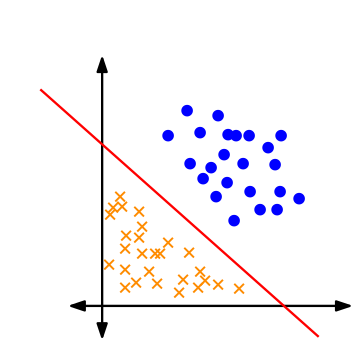
\includegraphics[width=\textwidth]{hiperplano_SVM_linear}
\caption{Linear. \label{fig:classificacao_dados:hiperplano_SVM_linear}}
\end{subfigure}
\begin{subfigure}[!ht]{0.3\textwidth}
	\centering
	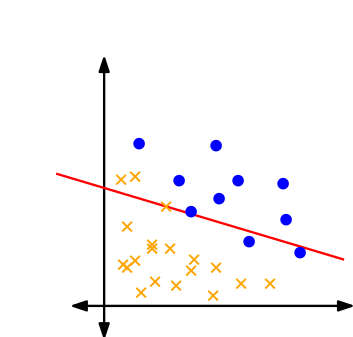
\includegraphics[width=\textwidth]{hiperplano_SVM_flexivel}
	\caption{Flexível. \label{fig:classificacao_dados:hiperplano_SVM_flexivel}}
\end{subfigure}
\begin{subfigure}[!ht]{0.3\textwidth}
	\centering
	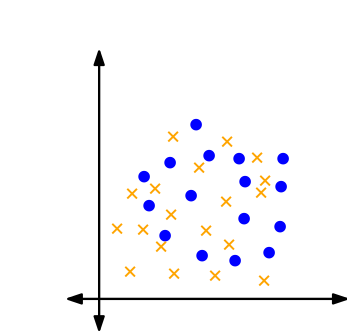
\includegraphics[width=\textwidth]{hiperplano_SVM_nao_linear}
	\caption{Não Linear. \label{fig:classificacao_dados:hiperplano_SVM_nao_linear}}
\end{subfigure}
\caption{Dados lineares, com margem flexível e não lineares. \label{fig:classificacao_dados}}
\end{figure}

Observe que na \Cref{fig:classificacao_dados:hiperplano_SVM_linear} os dados podem ser classificados corretamente através de uma reta. Já na \Cref{fig:classificacao_dados:hiperplano_SVM_flexivel} é possível encontrar uma reta que separa alguns poucos dados, porém incorretamente. E na \Cref{fig:classificacao_dados:hiperplano_SVM_nao_linear} não é possível classificar os dados como nos casos anteriores. Nestes exemplos temos representados os três casos de SVM: o linear com margem rígida, o linear com margem flexível e o não linear, respectivamente.

A modelagem do problema de classificação, utilizando a técnica de SVM, consiste em encontrar um hiperplano ótimo que melhor separe os dados de entrada $x^i$ em duas saídas $y_i$ através de uma função de decisão. Matematicamente, mostraremos que trata-se um problema de programação quadrática convexa com restrições lineares, que pode ser formulado como
\[
\begin{aligned}
\min_{w,b} & \quad f(w) \\
\text{s.a.} &  \quad g(w,b) \leq 0, \end{aligned}
\]
com $w\in \RR^n$ e $b\in \RR $, em que $f: \RR^n \rightarrow \RR$ é uma função quadrática e $g: \RR^{n+1} \rightarrow \RR^m$ é linear afim. Por consequência, $f$ e $g$ são continuamente diferenciáveis.



Para formular matematicamente o problema de classificação, considere os conjuntos de entrada $\Xset =\{x^1, \ldots , x^m \} \subset \RR^n$ e de treinamento $\Yset=\{(x^1, y_1), \ldots , (x^m, y_m)\mid x^i \in \Xset \, e \, y_i \in \{-1,1\}\}$, com a partição 
\[ \label{conj1}
\Xset ^{+} =\{x^i \in \Xset\mid y_i=1\} \quad e \quad \Xset^{-}=\{x^i \in \Xset\mid y_i=-1\},
\]
dos conjuntos formados pelos atributos pertencentes às classes positiva e negativa, respectivamente.

\begin{defi} Considere um vetor não nulo $w\in \RR^n$ e um escalar $b\in \RR$. Um \emph{hiperplano com vetor normal $w$ e constante $b$} é um conjunto da forma $\Hset(w,b)=\{x\in \RR^n \mid w^{T}x+b=0\}$.
\end{defi}

O hiperplano $\Hset(w,b)$ divide o espaço $\RR^n$ em dois semiespaços, dados por
\[ \label{conj2}
\mathcal{S}^{+}=\{x\in \RR^n \mid w^{T}x+b\geq 0\} \quad e \quad \mathcal{S}^{-}=\{x\in \RR^n \mid w^{T}x+b\leq 0\}.
\]


Considere dois conjuntos de dados de treinamento representados no $\RR^2$ como na \Cref{fig:dados_e_hiperplanos:dados_treinamento}, em que os pontos em azul representam a classe positiva, e os pontos em vermelho a classe negativa. Perceba na \Cref{fig:dados_e_hiperplanos:hiperplanos_separadores} que todos os hiperplanos representados separam corretamente os dados, porém nosso objetivo será encontrar o hiperplano que melhor separa esses dados, o qual está representado na \Cref{fig:dados_e_hiperplano_otimo:hiperplano_otimo} pela cor violeta. Logo, desejamos encontrar o hiperplano que possibilita a maior faixa que não contém nenhum dado, pois caso a faixa seja muito estreita pequenas perturbações no hiperplano ou no conjunto de dados podem resultar uma classificação incorreta. 
\begin{figure}[htbp] 
	\centering
	\begin{subfigure}[h]{0.38\textwidth}
		\centering
		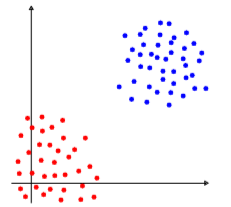
\includegraphics[width=\textwidth]{dados_treinamento}
		\caption{Dados de treinamento. \label{fig:dados_e_hiperplanos:dados_treinamento}}
	\end{subfigure}
	\begin{subfigure}[h]{0.38\textwidth}
		\centering
		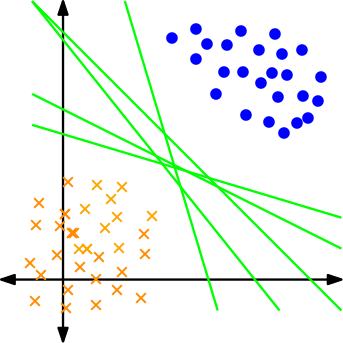
\includegraphics[width=\textwidth]{hiperplanos_separadores}
		\caption{Hiperplanos separadores. \label{fig:dados_e_hiperplanos:hiperplanos_separadores}}
	\end{subfigure}
\caption{Conjunto de Dados e Hiperplanos. \label{fig:dados_e_hiperplanos}}
\end{figure}
\begin{figure}[hbtp] 
	\centering
	\begin{subfigure}[h]{0.38\textwidth}
		\centering
		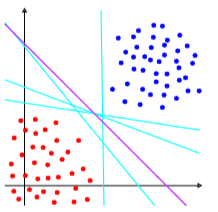
\includegraphics[width=\textwidth]{hiperplano_otimo}
		\caption{Hiperplano ótimo. \label{fig:dados_e_hiperplano_otimo:hiperplano_otimo}}
	\end{subfigure}
	\begin{subfigure}[h]{0.40\textwidth}
		\centering
		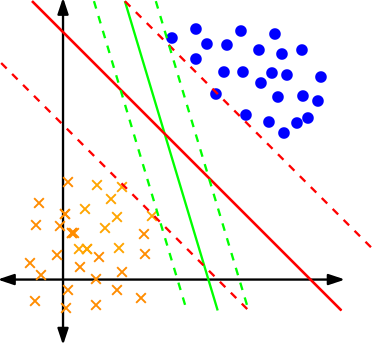
\includegraphics[width=\textwidth]{hiperplano_maxima_margem}
		\caption{Máxima margem. \label{fig:dados_e_hiperplano_otimo:hiperplano_maxima_margem}}	
	\end{subfigure}
\caption{Hiperplano Ótimo. \label{fig:dados_e_hiperplano_otimo}}
\end{figure}


\begin{defi} \label{def:dados_linearmente_separaveis} Os conjuntos $\Xset^{+}, \Xset^{-} \subset \RR^n$ são ditos \emph{linearmente separáveis} quando existem $w\in \RR^n$ e $b\in \RR$  tais que $w^{T}x+b>0$ para todo $x\in \Xset^{+}$ e $w^{T}x+b<0$ para todo $x\in \Xset^{-}$. O hiperplano $\Hset(w,b)$ é chamado hiperplano separador dos conjuntos $\Xset^{+}$ e $\Xset^{-}$.
\end{defi}


\begin{lema} \label{lema:hiperplanos_separadores} 
Suponha que os conjuntos $\Xset^{+}, \Xset^{-} \subset \RR^n$ são finitos e linearmente separáveis, com hiperplano separador $\Hset(w,b)$. Então, existem $\overline{w}\in \RR^n$ e $\overline{b}\in \RR$ tais que $\Hset(w,b)$ pode ser descrito por
\[
\wbar^{T}x+\bbar =0,
\]
satisfazendo
\begin{align}
\wbar^{T}x+\bbar &\geq 1, \text{ para todo } x\in \Xset^{+}, \label{eq:1_hiperplanos_separadores} \\
\wbar^{T}x+\bbar &\leq -1, \text{ para todo } x\in \Xset^{-}. \label{eq:2_hiperplanos_separadores}
\end{align}
\end{lema} 

\begin{proof}
Pela  \Cref{def:dados_linearmente_separaveis}, temos que existem $w\in \RR^n$ e $b\in \RR$ tais que
\begin{align}
w^{T}x+b &>0, \text{ para todo } x\in \Xset^{+}, \\
w^{T}x+b &<0, \text{ para todo } x\in \Xset^{-}.
\end{align}  

Como $\Xset^{+}\cup \Xset^{-}$ é um conjunto finito, podemos definir
\[ \boldsymbol{\gamma} \coloneqq \min_{x\in \Xset^{+}\cup \Xset^{-}} \vert w^{T}x+b\vert  >0. \]

Portanto, para todo $x\in \Xset^{+}\cup \Xset^{-}$, $\boldsymbol{\gamma} \leq \vert w^{T}x+b\vert$ e consequentemente, $\dfrac{\vert w^{T}x+b\vert }{\boldsymbol{\gamma}} \geq 1$. Assim, para $x\in \Xset^{+}$ temos
\[ \dfrac{w^{T}x+b}{\boldsymbol{\gamma}} = \dfrac{\vert w^{T}x+b\vert }{\boldsymbol{\gamma}} \geq 1, \]
e para $x\in \Xset^{-}$, temos
\[- \dfrac{w^{T}x+b}{\boldsymbol{\gamma}} = \dfrac{\vert w^{T}x+b\vert }{\boldsymbol{\gamma}} \geq 1. \]

Logo, definindo $\wbar \coloneqq \dfrac{w}{\boldsymbol{\gamma}}$ e $\bbar \coloneqq \dfrac{b}{\boldsymbol{\gamma}}$, obtemos as desigualdades \eqref{eq:1_hiperplanos_separadores} e \eqref{eq:2_hiperplanos_separadores}. 

\end{proof}


A partir do \Cref{lema:hiperplanos_separadores} podemos, sem perda de generalidade, considerar o hiperplano $\Hset (w,b)$, com $w$ e $b$ satisfazendo \eqref{eq:1_hiperplanos_separadores} e \eqref{eq:2_hiperplanos_separadores}. Além disso, temos que $\Hset^{+} (w,b) \coloneqq \{x\in \RR^n \mid w^{T}x+b= 1\}$ e $\Hset^{-} (w,b) \coloneqq \{x\in \RR^n \mid w^{T}x+b= -1\}$ são os hiperplanos que definem a faixa que separa os conjuntos $\Xset^{+}$ e $\Xset^{-}$.

\begin{prop} \label{prop:projecao_ortogonal_sobre_hiperplano} 
A projeção ortogonal de um vetor $\xbar\in \RR^n$ sobre um hiperplano afim $\Hset(w,b)$, é dada por
\[ \proj_{\Hset (w,b)}(\xbar)= \xbar - \dfrac{w^{T}\xbar+b}{w^{T}w}w. \]
Além disso, a $\proj_{\Hset (w,b)}(\xbar)$ satisfaz a menor distância.
\end{prop}

\begin{proof}
Sejam $w\in \RR^n$ o vetor normal ao hiperplano $\Hset(w,b)$, $\bar{z}\in \Hset(w,b)$ e $x^{*} \coloneqq \proj_{\Hset (w,b)}(\xbar)$ a projeção ortogonal de $\xbar$ sobre $\Hset(w,b)$. Assim, temos que 
\[ \label{eq:1_projecao_ortogonal_sobre_hiperplano} 
w^{T}(x^{*}-\bar{z})=0 
\]
e
\[ \label{eq:2_projecao_ortogonal_sobre_hiperplano} 
\xbar-x^{*}=\lambda w \Longrightarrow x^{*}=\xbar-\lambda w. 
\]
Substituindo \eqref{eq:2_projecao_ortogonal_sobre_hiperplano} em \eqref{eq:1_projecao_ortogonal_sobre_hiperplano}, obtemos
\begin{align}
0 &= w^{T}(\xbar-\lambda w-\overline{z}) \\
&= w^{T}\xbar-\lambda w^{T}w - w^{T}\bar{z}.
\end{align}
Resolvendo para $\lambda$ e como $w^{T}\bar{z} = -b$, temos
\[ \lambda =\dfrac{w^{T}\xbar-w^{T}\bar{z}}{w^{T}w} =\dfrac{w^{T}\xbar+b}{w^{T}w}. \]
Portanto, 
\[ x^{*}=\xbar-\dfrac{w^{T}\xbar+b}{w^{T}w}w . \]
Ademais, vamos provar que a $\proj_{\Hset (w,b)}(\xbar)$ satisfaz a menor distância, isto é,
\[ \Vert\xbar-x^{*}\Vert_{2} \leq \Vert \xbar-x\Vert_{2}, \]
para todo $x\in \Hset(w,b)$.
De fato, tomando $u=\xbar-x^{*}$ e $v=x^{*}-x$ observe que estes vetores são ortogonais, pois 
\begin{align}
u^{T}v&= (\xbar-x^{*})^{T}(x^{*}-x) \\
&= (\xbar-\xbar+\lambda w)^{T}(x^{*}-x) \\
&= \lambda w^{T}(x^{*}-x) \\
&= \lambda (w^{T}x^{*}-w^{T}x) \\
&= \lambda (-b-(-b)) \\
&= 0.
\end{align}
Assim, podemos utilizar Pitágoras, isto é, obtemos
\[ \Vert u+v\Vert^{2}=\Vert u\Vert^{2} + 2u^{T}v + \Vert v\Vert^{2}=\Vert u\Vert^{2} + \Vert v\Vert^{2} , \]
e utilizamos as definições de $u$ e $v$ para obter
\[ 
\Vert \xbar-x\Vert^{2}=\Vert \xbar-x^{*}\Vert^{2} + \Vert x^{*}-x\Vert^{2} \geq \Vert x^{*} - x \Vert^{2} . 
\]
\end{proof}


Utilizando a \Cref{prop:projecao_ortogonal_sobre_hiperplano} podemos demonstrar o \Cref{lema:distancia_entre_hiperplanos}, o qual estabelece a largura da faixa entre os hiperplanos separadores $\Hset^{+} (w,b)$ e $\Hset^{-} (w,b)$.

\begin{lema} \label{lema:distancia_entre_hiperplanos} 
A distância entre os hiperplanos $\Hset^{+} (w,b)$ e $\Hset^{-} (w,b)$ é dada por 
\[
\dist(\Hset^{+}, \Hset^{-})=\dfrac{2}{\Vert w\Vert}.
\] 
\end{lema}
\begin{proof}
Considere um ponto arbitrário $\xbar\in \Hset^{+} (w,b)$ e seja $x^{*}\in \Hset^{-} (w,b)$ a projeção ortogonal de $\xbar$ sobre $\Hset^{-} (w,b)$. Usando a \Cref{prop:projecao_ortogonal_sobre_hiperplano}, temos
\[ \label{eq:1_distancia_entre_hiperplanos} 
x^{*}= \proj_{\Hset^{-} (w,b)}(\xbar)= \xbar - \dfrac{w^{T}\xbar+b+1}{\Vert w\Vert^{2}}w. 
\] 
Além disso, a distância entre dois conjuntos é definida por
\[ 
\dist(\Hset^{+}, \Hset^{-}) \coloneqq  \inf\{\Vert x^{+}-x^{-} \Vert : x^{+}\in \Hset^{+} (w,b)\ \text{e} \ x^{-}\in \Hset^{-} (w,b) \},
\]
e como a $\proj_{\Hset^{-} (w,b)}(\xbar)$ satisfaz a menor distância entre $\xbar$ e $\Hset^{-} (w,b)$ e, $\Hset^{+} (w,b)$ é paralelo a $\Hset^{-} (w,b)$, temos que 
\[ \label{eq:2_distancia_entre_hiperplanos} 
\dist(\Hset^{+},\Hset^{-})=\Vert \xbar-x^{*}\Vert. 
\]

Substituindo \eqref{eq:1_distancia_entre_hiperplanos} em \eqref{eq:2_distancia_entre_hiperplanos} obtemos
\begin{align} 
\dist(\Hset^{+},\Hset^{-}) &= \Vert \xbar-x^{*}\Vert \\
&= \left\Vert \xbar -\xbar +\dfrac{w^{T}\xbar+b+1}{\Vert w\Vert^{2}}w \right\Vert \\
&=  \dfrac{\vert w^{T}\xbar+b+1 \vert}{\Vert w\Vert^{2}} \Vert w\Vert \\
&= \dfrac{\vert w^{T}\xbar+b+1 \vert}{\Vert w\Vert},
\end{align}
e como $\xbar\in \Hset^{+} (w,b)$,  $ w^{T}\xbar+b=1$ implica
\[  w^{T}\xbar =1-b, \]
concluindo que 
\begin{align} 
\dist(\Hset^{+},\Hset^{-})&= \dfrac{\vert 1-b+b+1 \vert}{\Vert w\Vert} \\
&= \dfrac{2}{\Vert w\Vert }. 
\end{align}
\end{proof}


%--------------------------------------------------------------------------------------------------------------------------


\subsection{Formulação Matemática do Problema de Classificação - Margem Rígida}

Encontrar o hiperplano que melhor separa os dados implica maximizar a largura da margem, isto é, maximizar $\dist(\Hset^{+} , \Hset^{-}) =\dfrac{2}{\Vert w\Vert }$. Isso equivale a minimizar seu inverso $\dfrac{1}{2}\Vert w\Vert $ ou ainda minimizar $\dfrac{1}{2}\Vert w\Vert^{2}$. De fato, seja $w^{*}=\argmax\dfrac{2}{\Vert w\Vert}$. Então, para todo $w\in \RR^n$,
\[ 
\dfrac{2}{\Vert w^{*}\Vert} \geq \dfrac{2}{\Vert w\Vert} 
\]
implica
\[ \label{eq:maximizar_distancia_equivalente_minimizar} 
\Vert w\Vert \geq \Vert w^{*}\Vert. 
\]
Logo, $w^{*} \in \argmin\Vert w\Vert$. Além disso, como $\Vert \cdot \Vert$ é não negativa, elevando ao quadrado ambos os lados da desigualdade \eqref{eq:maximizar_distancia_equivalente_minimizar} temos que  $\Vert w\Vert^{2} \geq \Vert w^{*}\Vert^{2}$ implica
\[ 
\dfrac{1}{2}\Vert w\Vert^{2} \geq \dfrac{1}{2}\Vert w^{*}\Vert^{2}. 
\]
Portanto, 
\[ \argmax\dfrac{2}{\Vert w\Vert} = \argmin\dfrac{1}{2}\Vert w\Vert^2. \]

Ademais, como a faixa deve separar os dados das duas classes, as seguintes restrições devem ser satisfeitas
\begin{align}
w^{T}x+b &\geq 1 , \text{ para  todo } x\in \Xset^{+}, \\
w^{T}x+b &\leq -1 , \text{ para  todo } x\in \Xset^{-}.
\end{align}

Considerando que $\Xset^{+}=\{x^i \in \Xset\mid y_i=1\}$ e $\Xset^{-}=\{x^i \in \Xset \mid y_i=-1\}$, podemos reescrever as restrições acima de uma forma mais compacta 
\[ y_{i}(w^{T}x^{i}+b)\geq 1, \quad i=1, \ldots ,m. \]

Portanto, o problema de encontrar o hiperplano ótimo pode ser formulado da seguinte maneira
\[ \label{eq:problemageralSVM}
\begin{aligned}
\min_{w,b} & \quad \dfrac{1}{2} \Vert w\Vert^{2} \\
\text{s.a.} &  \quad y_i(w^{T}x^{i}+b) \geq 1, \quad i=1, \ldots , m, \end{aligned}
 \]
em que $w\in \RR^{n}$ e $b\in \RR$. 

O problema \eqref{eq:problemageralSVM} possui função objetivo 
\[ f(w,b)=\dfrac{1}{2}\Vert w\Vert^{2} \]
convexa, e restrições lineares (DEMONSTRAR)
\[ g_i(w,b)=1-y_i(w^{T}x^{i}+b) \leq 0, \quad i=1, \ldots, m, \]
em que a função $g:\RR^{n+1} \rightarrow \RR^{m}$ pode ser escrita da forma 
\[ g(w,b)= e - (YX^{T}w+by) \leq 0, \]
com $e$ sendo o vetor cujas $m$ componentes são todas iguais a $1$, $Y=\diag(y_{i})$, $X=\diag(x^{i})$, $y^{T}=[y_{1} \ \ldots \ y_{m}]$, $w\in \RR^n$ e $b\in \RR$.


%----------------------------------------------------------------------------------------------------------------------

\subsection{Formulação Matemática do Problema de Classificação - Margem Flexível (CSVM)}

Situações reais dificilmente envolvem problemas cujos dados são linearmente separáveis. Em vista disso, faz-se necessário estender os conceitos e resultados estudados nas SVMs lineares de margem rígida para o caso de SVM com margem flexível, quando os dados não são linearmente separáveis. Para tanto, considere um conjunto de dados não-linearmente separável como da \Cref{fig:dados_linearmente_separaveis_e_nao_separaveis:b}, isto é, não existe um hiperplano separador. 


\begin{figure}[htbp] 
	\centering
	\begin{subfigure}[h]{0.30\textwidth}
		\centering
		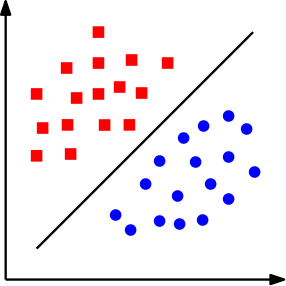
\includegraphics[width=\textwidth]{dados_linearmente_separaveis}
		\caption{Dados linearmente separáveis. \label{fig:dados_linearmente_separaveis_e_nao_separaveis:a}}
	\end{subfigure}
	\begin{subfigure}[h]{0.30\textwidth}
		\centering
		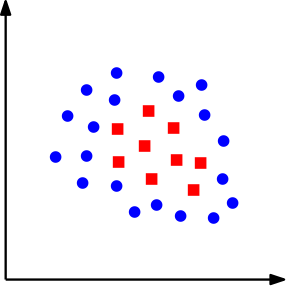
\includegraphics[width=\textwidth]{dados_nao_linearmente_separaveis}
		\caption{Dados não-linearmente separáveis. \label{fig:dados_linearmente_separaveis_e_nao_separaveis:b}}
	\end{subfigure}
\caption{Conjunto de dados. \label{fig:dados_linearmente_separaveis_e_nao_separaveis} }
\end{figure}


Neste caso, temos que o conjunto viável
\[
\{ (w,b) \in \RR^{n+1} \mid 1-y_{i}(w^{T}x^{i} + b) \leq 0 , \quad i=1, \ldots , m \}
\]
é vazio e, portanto, a formulação dada pelo problema \eqref{eq:problemageralSVM} não fornece um classificador.

Assim, no intuito de contornar esse problema utilizamos regularização para suavizar as margens, acrescentando variáveis de folga $\xi_{i} \geq 0$ associadas aos dados de treinamento $x_{i}$, com $i=1, \ldots , m$, e permitindo, assim, uma flexibilização do problema de estimar as variáveis $w$ e $b$. Em outras palavras, a restrição $1-y_{i}(w^{T}x^{i} + b) \leq 0$ é relaxada e substituída por $1-y_{i}(w^{T}x^{i} + b) \leq \xi_{i} $, com $\xi_{i} \geq 0$. Cada variável de folga $\xi_{i}$ mensura a distância que determinado dado $x_{i}$ está do seu respectivo hiperplano separador, caso este dado esteja do lado errado.

%Esta imagem também não está sendo lida, detectar problema #chateada -Uhhhul deu certo! LEMBRETE: não usar acento ao nomear figuras
\begin{figure}[!ht] 
	\centering
	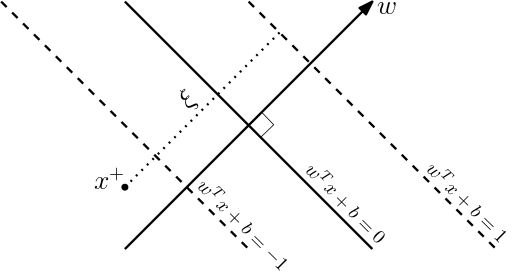
\includegraphics[width=0.50\textwidth]{variaveis_de_folga}
	\caption{Variáveis de folga. \label{fig:variaveis_de_folga}}
\end{figure}

Tal procedimento permite que pontos da classe positiva permaneçam fora do semiespaço $\mathcal{S}^{+}=\{x\in \RR^n \mid w^{T}x+b\geq 1\}$ ou pontos da classe negativa fora do semiespaço $\mathcal{S}^{-}=\{x\in \RR^n \mid w^{T}x+b\leq -1\}$. 

Nesta formulação o hiperplano separador é denominado hiperplano de margem flexível e as restrições dos hiperplanos separadores são reformuladas da seguinte maneira 
\begin{align}
w^{T}x^{i}+b &\geq 1 - \xi_{i} , \text{ para  todo } x^{i} \in \Xset^{+}, \label{restricoesCSVM+} \\
w^{T}x^{i}+b &\leq -1 +\xi_{i} , \text{ para  todo } x^{i} \in \Xset^{-}. \label{restricoesCSVM-}
\end{align}


Agora nosso objetivo é encontrar $w$ e $b$ ótimos de modo a obter um bom classificador. Primeiramente, observe que dados $w$ e $b$ arbitrários, podemos escolher $\xi_{i} \geq 0$ de modo que as restrições \eqref{restricoesCSVM+} e \eqref{restricoesCSVM-} sejam satisfeitas. Para tanto, podemos definir
\[
\xi_{i} =  \left \{ \begin{array}{cc} \max\{0, 1-w^{T}x^{i}-b\}, & \quad \text{se} \quad x^{i} \in \Xset^{+}, \\
\max\{0, 1+w^{T}x^{i}+b\}, & \quad \text{se} \quad x^{i} \in \Xset^{-}.
\end{array} \right .
\]
 
Desse modo, para obter um bom classificador não basta apenas maximizar a margem definida pelos hiperplanos $\Hset^{+} (w,b)$ e $\Hset^{-} (w,b)$ e introduzir as variáveis de folga nas restrições, mantendo a mesma função objetivo, pois, como exemplificado por \textcite{Evelin2017}, a \Cref{fig:hiperplano_nao_classificador} ilustra o hiperplano dado por $w_{0}^{T}x+b = 0$, que não poder ser usado para classificar os dados, mas satisfaz as restrições \eqref{restricoesCSVM+} e \eqref{restricoesCSVM-}. 

\begin{figure}[!ht] 
	\centering
	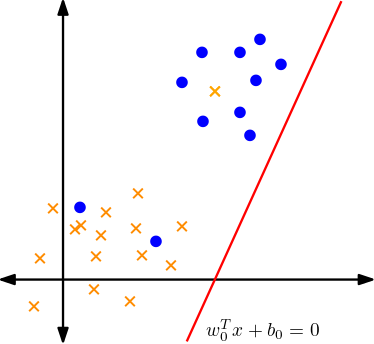
\includegraphics[width=0.38\textwidth]{hiperplano_nao_classifica_dados}
	\caption{Exemplo de hiperplano que não classifica os dados. \label{fig:hiperplano_nao_classificador}}
\end{figure}
 

Portanto, para reformular o problema original de maximizar a margem é preciso também controlar o valor dessas variáveis de modo a estimular uma classificação correta, pois quanto maior o valor delas mais será permitido violar as restrições. Em vista disso, é acrescentada na função objetivo uma parcela que corresponde à penalização das violações e o problema \eqref{eq:problemageralSVM} é reformulado da seguinte forma

\[ \label{eq:problemaCSVM}
\begin{aligned}
\min_{w,b,\xi} & \quad \dfrac{1}{2} \Vert w\Vert^{2} + C \sum_{i=1}^{m} \xi_{i} \\
\text{s.a.} &  \quad y_i(w^{T}x^{i}+b) \geq 1 - \xi_{i}, \quad i=1, \ldots , m, \\
& \xi_{i} \geq 0, \quad i=1, \ldots , m,\end{aligned}
\]
%não consegui alinhar a última linha às duas primeiras
em que $C>0$ é um parâmetro de regularização que tem o objetivo de controlar a importância das variáveis de folga. O valor do parâmetro $C$ que fornece uma boa classificação dos dados é escolhido de maneira heurística na fase de treinamento, geralmente a partir da natureza do problema.É devido a utilização desse parâmetro esta modelagem de SVM também é conhecida como C-SVM.

O termo $C \sum_{i=1}^{m} \xi_{i}$ na função objetivo do problema \eqref{eq:problemaCSVM} pode ser pensado como uma medida de erro de classificação, pois minimiza o valor das variáveis de folga e reduz desse modo o número de pontos classificados incorretamente. De fato, aumentando o valor do parâmetro $C$ aumenta-se a penalização sobre a violação da restrição original do problema SVM. Por outro lado, diminuindo o valor de $C$ o modelo se torna mais flexível a esse tipo de violação. 

O problema de margem flexível \eqref{eq:problemaCSVM}, assim como o problema \eqref{eq:problemageralSVM}, também possui restrições lineares 
\begin{align} 
g_{i}(w,b,\xi) = & 1-\xi_{i} - y_i(w^{T}x^{i}+b) \leq 0 \quad \text{e} \\
h_{i}(w,b,\xi) = & - \xi_{i} \leq 0, \quad i=1, \ldots, m,
\end{align}

e assim, o conjunto factível
\[
\Omega = \{(w,b,\xi) \in \RR^{n+1+m} \mid g_{i}(w,b,\xi) \leq 0, \, h_{i}(w,b,\xi) \leq 0, \, i=1, \ldots, m \} 
\]
é um poliedro não vazio.

Ademais, a função objetivo $f$ é quadrática e limitada inferiormente em $\Omega$, pois 
\[
f(w,b,\xi) = \dfrac{1}{2} \Vert w\Vert^{2} + \underbrace{C}_{> 0} \sum_{i=1}^{m} \underbrace{\xi_{i}}_{\geq 0} \geq 0.
\]

%Assim o Teorema de Programação Quadrática (1.34) garante a existência de um minimizador global para o problema \eqref{eq:problemaCSVM}.


%-------------------------------------------------------------------------------------------------------------------------

\newpage
\section{Conceitos de Otimização} \label{chap:conceitos_de_otimizacao}


Tendo em vista que o problema de classificação trata-se de um problema de Otimização, neste capítulo pretendemos discutir alguns conceitos e resultados para o problema 
\[ \label{problema_geral_otimizacao}
\begin{aligned}
\min_{x} & \quad f(x) \\
\text{s.a} & \quad x \in \Omega ,
\end{aligned}
\]
em que $f: \RR^{n} \rightarrow \RR$ é chamada \emph{função objetivo}, $\Omega \subset \RR^{n}$ é chamado \emph{conjunto factível} do problema \eqref{problema_geral_otimizacao} e os pontos de $\Omega$ são chamados de \emph{pontos factíveis}. Para o desenvolvimento deste capítulo, em particular da teoria de otimização irrestrita, as principais referências utilizadas foram \textcite{Izmailov2014ac,Ademir2013}. Já os conceitos e resultados da teoria de otimização com restrições foram desenvolvidos, principalmente, com base em \textcite{Ana1994,luenberger2008linear}.  

Inicialmente, faz-se necessário caracterizar os pontos que são solução do problema \eqref{problema_geral_otimizacao}.

\begin{defi} \label{defi:minimizador_local_global}
Dizemos que um ponto $x^{*} \in \Omega$ é
\begin{enumerate}
	\item[(a)] \emph{minimizador local} de $f$ em $\Omega$ se, e somente se, existe $\varepsilon >0$ tal que $f(x^{*}) \leq f(x)$ para todo $x \in B(x^{*}, \varepsilon) \cap \Omega$.

	\item[(b)] \emph{minimizador global} de $f$ em $\Omega$ se, e somente se, $f(x^{*}) \leq f(x)$ para todo $x \in \Omega$
\end{enumerate} 
\end{defi}

Quando as desigualdades na \Cref{defi:minimizador_local_global} forem estritas para $x \neq x^{*}$, diremos que $x^{*}$ é minimizador estrito. Essas definições são representadas na \Cref{fig:grafico_minimo_local_global}.

\begin{figure}[!ht] 
	\centering
	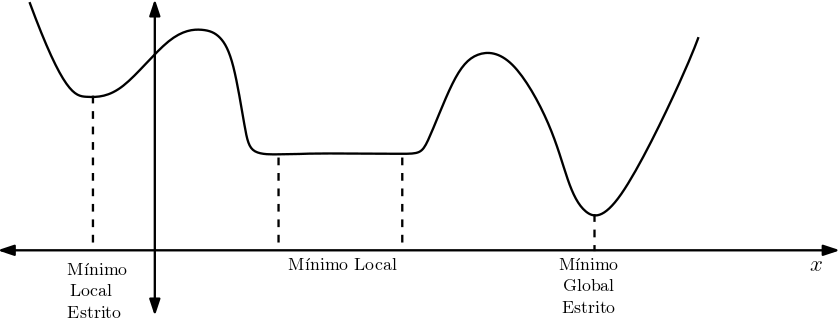
\includegraphics[width=0.86\textwidth]{grafico_minimo_local_global}
	\caption{ Mínimo local e mínimo global em uma dimensão. \label{fig:grafico_minimo_local_global}}
\end{figure}

Pela \Cref{defi:minimizador_local_global}, todo minimizador global é também minimizador local, porém a recíproca não é verdadeira. É interessante salientar que em muitas circunstâncias iremos nos contentar com um ponto de mínimo local pois, de modo geral, condições globais e soluções globais só podem ser encontradas se o problema possuir certas propriedades que garantem, essencialmente, que qualquer mínimo local é global. Uma destas propriedades é a convexidade, a qual abordaremos mais adiante (veja \Cref{chap:otimizacao_convexa}).

\begin{obs}
Todo problema de maximização
\[
\begin{aligned}
\max_{x} & \quad f(x) \\
\text{s.a} & \quad x \in \Omega \end{aligned}
 \]
pode ser transformado em um problema de minimização equivalente
\[
\begin{aligned}
\min_{x} & \quad -f(x) \\
\text{s.a} & \quad x \in \Omega .\end{aligned}
\]
Em particular, as soluções locais e globais de ambos os problemas são as mesmas, com sinais opostos para os valores ótimos.
\end{obs} %acrescentar imagem izmailoz&solodov

%Se a função objetivo $f$ for linear, \eqref{problema_geral_otimizacao} é chamado de problema de \emph{programação linear}, e se $f$ for uma função quadrática, \eqref{problema_geral_otimizacao} é chamado de problema de \emph{programação quadrática}. Ademais, quando $\Omega$ é um conjunto convexo e $f$ é uma função convexa, dizemos que \eqref{problema_geral_otimizacao} é um problema de \emph{programação convexa}. 


Ademais, quando o conjunto factível $\Omega = \RR^{n}$ dizemos que o problema \eqref{problema_geral_otimizacao} é irrestrito. No caso em que $\Omega$ é definido por um sistema de igualdades ou desigualdades como
\[
\Omega = \{ x\in \RR^{n} \mid h(x)=0, g(x) \leq 0 \},
\]
falamos em otimização com restrições.

Frequentemente, a formulação de problemas mais complexos envolve restrições à função objetivo. No entanto, veremos mais adiante que muitos desses problemas podem ser convertidos em problemas irrestritos, utilizando as restrições para estabelecer relações entre as variáveis. Em vista disso, abordaremos primeiramente a teoria de otimização para o caso irrestrito para posteriormente obter as condições de otimalidade para problemas com restrições de igualdade e desigualdade, haja vista que o problema de classificação, o qual estamos interessados em resolver, possui tal formato.

\begin{defi} \label{defi:valor_otimo}
Dizemos que $\bar{v} \in \RR \cup \{ -\infty \}$ definido por
\[
\bar{v} = \inf_{x \in \Omega} f(x)
\]
é o \emph{valor ótimo} do problema \eqref{problema_geral_otimizacao}.
\end{defi}

No estudo do problema de otimização irrestrita uma das principais questões que surge diz respeito a existência da solução. Observe que se na \Cref{defi:valor_otimo} temos $\bar{v} = - \infty$, o problema \eqref{problema_geral_otimizacao} não admite solução global, pois neste caso $f$ é ilimitada inferiormente no conjunto factível. Outro caso em que também não existe minimizador global ocorre quando $\bar{v}$ não é atingido em nenhum ponto factível. Vejamos um exemplo.

\begin{exem}
Seja $f: \RR \rightarrow \RR$, definida por $f(x) = e^{x}$, $\Omega = \RR$. Note que $\bar{v} = \inf_{x \in \RR} e^{x} = 0$, contudo, não existe $x \in \RR$ tal que $e^{x} = 0$. 
De modo análogo, considere $f$ definida como anteriormente e $\Omega = (0,1]$. Temos que $\bar{v} = \inf_{x \in (0,1]} e^{x} = 1$ e novamente não existe $x \in (0,1]$ tal que $e^{x}=1$. Observe que a função $f$ é contínua em $\Omega$, porém no primeiro caso $\Omega$ não é limitado e no segundo, $\Omega$ não é fechado. 
Considere agora $\Omega = [0,1]$, $f(x)=e^{x}$ para $x \in (0,1]$ e $f(0)=0$. Novamente, $\bar{v} = \inf_{x \in (0,1]} e^{x} = 1$, porém não existe $x\in \Omega$ tal que $f(x)=1$. Neste exemplo, $\Omega$ é compacto mas $f$ não é contínua.
\end{exem}

Assim, a partir desses exemplos é possível perceber que a existência de soluções está relacionada à continuidade da função objetivo e à compacidade do conjunto factível. O principal resultado que garante a existência de soluções globais é o Teorema de Weierstrass.

\begin{teo}(\textbf{Weierstrass}) \label{teo:weierstrass}
Sejam $f: \RR^{n} \rightarrow \RR$ uma função contínua e $\Omega \in \RR^{n}$ um conjunto compacto não vazio. Então existe minimizador global de $f$ em $\Omega$.
\end{teo}
\begin{proof}
A imagem de um conjunto compacto por uma função contínua é compacta. Assim, $f(\Omega)$ é compacto, em particular, como $f(\Omega) \in \RR$, este conjunto é limitado inferiormente, ou seja, existe $\bar{v} \in \RR$ tal que
\[
\bar{v} = \inf_{x\in \Omega} f(x).
\]
Pela definição de ínfimo, temos que para todo $k\in \mathds{N}$ existe $x^{k} \in \Omega$ tal que 
\[
\bar{v} \leq f(x^{k}) \leq \bar{v} + \dfrac{1}{k} .
\]
Passando ao limite quando $k \rightarrow \infty $, e usando o Teorema do Sanduíche concluímos que
\[\label{eq:teo_weierstrass}
\lim_{k \rightarrow \infty} f(x^{k}) = \bar{v}.
\]
Como $\{ x^{k} \} \in \Omega$ e $\Omega$ é compacto, temos que $\{ x^{k} \}$ é uma sequência limitada. Logo, ela possui uma subsequência convergente em $\Omega$, isto é, existe uma subsequência $\{ x^{k_{j}} \}$ que converge para um ponto $\bar{x} \in \Omega$,
\[
\lim_{j \rightarrow \infty} x^{k_{j}} = \bar{x} \in \Omega .
\]
Como $f$ é contínua, temos que
\[
\lim_{j \rightarrow \infty} f(x^{k_{j}}) = f(\bar{x}).
\]
Usando \eqref{eq:teo_weierstrass}, temos que $f(\bar{x}) = \bar{v}$ e portanto, $f$ assume valor mínimo no ponto $\bar{x} \in \Omega$. Em outras palavras, $\bar{x}$ é um minimizador global de $f$ em $\Omega$.
\end{proof}


\subsection{Condições de Otimalidade para Problemas sem Restrições} \label{subsection:irrestrito}

Considere o problema \eqref{problema_geral_otimizacao} irrestrito , isto é, com $\Omega = \RR^{n}$,
\[ \label{problema_otimizacao_irrestrita}
\begin{aligned}
\min_{x} & \quad f(x) \\
\text{s.a} & \quad x \in \RR^{n} ,
\end{aligned}
\]
em que $f:\RR^{n} \rightarrow \RR$. Nesta seção serão determinadas as condições que um ponto $x^{*} \in \RR^{n}$ deve satisfazer quando é minimizador local do problema \eqref{problema_otimizacao_irrestrita}. Condições desse tipo são chamadas de \emph{condições necessárias de otimalidade}. Determinaremos também as condições que garantem que um ponto dado é minimizador local do problema, que são denominadas \emph{condições suficientes de otimalidade}. 

Para os resultados que vem a seguir vamos utilizar os \Cref{fato:Taylor_primeira_ordem,fato:Taylor_segunda_ordem}, que fornecem a Fórmula de Taylor de primeira e segunda ordem. As demonstrações destes fatos podem ser encontradas em \textcite[p.194]{Elon2019}.


\begin{fato}(\textbf{Taylor de Primeira Ordem}) \label{fato:Taylor_primeira_ordem}
Seja $f:\RR^{n} \rightarrow \RR$ uma função diferenciável e $\xbar \in \RR^{n}$. Então podemos escrever
\[
f(x) = f(\xbar) + \nabla f(\xbar)^{T}(x-\xbar) + o(x),
\]
com $\lim_{x \rightarrow \xbar}\dfrac{o(x)}{\Vert x-\xbar \Vert} = 0$.
\end{fato}

\begin{fato}(\textbf{Taylor de Segunda Ordem}) \label{fato:Taylor_segunda_ordem}
Seja $f:\RR^{n} \rightarrow \RR$ uma função duas vezes diferenciável e $\xbar \in \RR^{n}$. Então
\[
f(x) = f(\xbar) + \nabla f(\xbar)^{T}(x-\xbar) + \dfrac{1}{2}(x-\xbar)^{T}\nabla^{2} f(\xbar)(x-\xbar) + o(x),
\] 
com $\lim_{x \rightarrow \xbar}\dfrac{o(x)}{\Vert x - \xbar \Vert^{2}} = 0$.
\end{fato}

Agora, nos teoremas que seguem, mostraremos as condições de otimalidade de primeira e de segunda ordem para o problema irrestrito.

\begin{teo}(\textbf{Condição necessária de primeira ordem}) \label{teo:condicao_necessaria_1_ordem}
Seja $f:\RR^{n} \rightarrow \RR$ diferenciável no ponto $x^{*} \in \RR^{n}$. Se $x^{*}$ é um minimizador local de $f$, então
\[ \label{eq:condicao_necessaria_1_ordem}
\nabla f(x^{*}) = 0.
\]
\end{teo}
\begin{proof}
Considere $d \in \RR^{n}$ arbitrário, porém fixo. Pela definição de minimizador local, existe $\varepsilon > 0$ tal que 
\[ \label{eq:1_condicao_1_ordem_irrestrito}
f(x^{*}) \leq f(x^{*}+td),
\]
para todo $t\in (0,\varepsilon ]$. Pela diferenciabilidade de $f$ em $x^{*}$, aplicando o \Cref{fato:Taylor_primeira_ordem}, podemos escrever 
\[
f(x^{*}+td) = f(x^{*}) + t\nabla f(x^{*})^{T}d + o(t),
\] 
com $\lim_{t\rightarrow 0} \dfrac{o(t)}{t} =0$. Utilizando \eqref{eq:1_condicao_1_ordem_irrestrito}, temos
\[
0 \leq t\nabla f(x^{*})^{T}d + o(t),
\]
e dividindo por $t>0$, 
\[
0 \leq \nabla f(x^{*})^{T}d + \dfrac{o(t)}{t} .
\]
Passando o limite quando $t\rightarrow 0$, obtemos
\[
0 \leq \nabla f(x^{*})^{T}d .
\]
Supondo que $\nabla f(x^{*})$ fosse não-nulo, como $d \in \RR^{n}$ é arbitrário, poderíamos escolher $d=-\nabla f(x^{*})$, resultando em
\[
0 \leq \nabla f(x^{*})^{T}d = - \Vert \nabla f(x^{*}) \Vert^{2} ,
\]
o que é uma contradição. Portanto, $\nabla f(x^{*}) =0$.
\end{proof}


\begin{defi}\label{defi:ponto_critico}
Um ponto $x^{*} \in \RR^{n}$ que cumpre a condição \eqref{eq:condicao_necessaria_1_ordem} é dito \emph{ponto crítico} ou \emph{estacionário} da função $f$. 
\end{defi}


%retirado do texto:a matriz Hessiana de $f$ no ponto $x^{*}$ é semidefinida positiva, isto é,
\begin{teo}(\textbf{Condição necessária de segunda ordem}) \label{teo:condicao_necessaria_2_ordem}
Seja $f:\RR^{n} \rightarrow \RR$ duas vezes diferenciável no ponto $x^{*} \in \RR^{n}$. Se $x^{*}$ é um minimizador local de $f$, então 
\[
d^{T} \nabla^{2} f(x^{*})d \geq 0,
\]
para todo $d \in \RR^{n}$.
\end{teo}
\begin{proof}
Seja novamente $d\in \RR^{n}$ arbitrário, porém fixo. Se $x^{*}$ é minimizador local de $f$, então para todo $t>0$ suficientemente pequeno, temos que
\[\label{eq:1_condicao_2_ordem_irrestrito}
0 \leq f(x^{*}+td) - f(x^{*}).
\]
Aplicando o \Cref{fato:Taylor_segunda_ordem},
\[
f(x^{*}+td) = f(x^{*}) + t\nabla f(x^{*})^{T}d + \dfrac{t^{2}}{2} d^{T}\nabla^{2} f(x^{*})d + o(t^{2}),
\]
com $\lim_{t\rightarrow 0} \dfrac{o(t^{2})}{t^{2}} =0$, e  \eqref{eq:1_condicao_2_ordem_irrestrito} implica em
\[ \label{eq:2_condicao_2_ordem_irrestrito}
0 \leq \dfrac{t^{2}}{2} d^{T}\nabla^{2} f(x^{*})d + o(t^{2}),
\]
 pois como $x^{*}$ é minimizador local, o \Cref{teo:condicao_necessaria_1_ordem} garante que $\nabla f(x^{*}) =0$. Dividindo ambos os lados da desigualdade \eqref{eq:2_condicao_2_ordem_irrestrito} por $t^{2}$ e tomando o limite quando $t\rightarrow 0$, obtemos
\[
d^{T} \nabla^{2} f(x^{*})d \geq 0,
\]
para todo $d \in \RR^{n}$.
\end{proof}

\begin{defi} \label{defi:definida_positiva}
Seja $A \in \RR^{n\times n}$ uma matriz simétrica. Dizemos que $A$ é \emph{definida positiva} quando $x^{T}Ax >0$, para todo $x\in \RR^{n}$, $x \neq 0$. Tal propriedade é denotada por $A \succ 0$. Se $x^{T}Ax \geq 0$, para todo $x\in \RR^{n}$, $A$ é dita \emph{semidefinida positiva}, fato este denotado por $A \succcurlyeq 0$.
\end{defi}
\begin{obs}
A definição geral de positividade de uma matriz não exige que ela seja simétrica. Entretanto, neste trabalho sempre que dissermos que a matriz é definida ou semidefinida positiva assumimos implicitamente que a matriz é simétrica.
\end{obs}

Assim, de acordo com a \Cref{defi:definida_positiva}, o \Cref{teo:condicao_necessaria_2_ordem} nos diz que se um ponto $x^{*}$ é minimizador local de $f$, então a matriz Hessiana $\nabla^{2} f(x^{*})$ é semidefinida positiva.

É possível obter, a partir da condição necessária de segunda ordem, a condição suficiente de segunda ordem, isto é, condição que implica que $x^{*}$ é minimizador local estrito, bastando para isso pedir a definição positiva da Hessiana.

\begin{teo}(\textbf{Condição suficiente de segunda ordem}) \label{teo:condicao_suficiente_irrestrito}
Seja $f:\RR^{n} \rightarrow \RR$ duas vezes diferenciável no ponto $x^{*} \in \RR^{n}$. Se $x^{*}$ é um ponto estacionário da função $f$ e $\nabla^{2} f(x^{*})$ é definida positiva, então $x^{*}$ é minimizador local estrito de $f$.
\end{teo}
\begin{proof}
Seja $B \coloneqq \{ h\in \RR^{n} \mid \Vert h \Vert =1 \}$ e consideremos a função $\phi : B \rightarrow \RR$ dada por
\[
\phi (h) = h^{T} \nabla^{2} f(x^{*})h.
\]
A função $\phi$ é contínua e $B$ é um conjunto compacto, portanto, pelo \Cref{teo:weierstrass}, $\phi$ atinge um valor máximo e um valor mínimo em $B$. Considere $a = \phi(h^{*})$ o valor mínimo de $\phi$ em $B$. Como $\nabla^{2} f(x^{*}) \succ 0$, então $\phi(h) >0$, para todo $h\in B$ e, em particular,
\[
\phi(h) \geq a >0.
\]
Agora, consideremos $d\in \RR^{n}$, arbitrário não-nulo. Como $\dfrac{d}{\Vert d \Vert} \in B$, temos que
\[
{\dfrac{d}{\Vert d \Vert}}^{T} \nabla^{2} f(x^{*})\dfrac{d}{\Vert d \Vert} \geq a
\]
implica em
\[ \label{eq:1_condicao_suficiente_irrestrito}
d^{T}\nabla^{2} f(x^{*})d \geq a\vert d\Vert^{2} .
\]
Aplicando o \Cref{fato:Taylor_segunda_ordem} em torno de $x^{*}$, temos
\[\label{eq:2_condicao_suficiente_irrestrito}
f(x^{*}+d) - f(x^{*}) = \nabla f(x^{*})^{T}d + \dfrac{1}{2} d^{T}\nabla^{2} f(x^{*})d + o(\Vert d \Vert^{2}).
\]
Como, por hipótese, $\nabla f(x^{*}) = 0$, \eqref{eq:1_condicao_suficiente_irrestrito} e \eqref{eq:2_condicao_suficiente_irrestrito} implicam que
\[ 
f(x^{*}+d) - f(x^{*}) = \dfrac{1}{2} d^{T}\nabla^{2} f(x^{*})d + o(\Vert d \Vert^{2}) ,
\]
e assim, 
\[ \label{eq:3_condicao_suficiente_irrestrito}
f(x^{*}+d) - f(x^{*}) \geq \dfrac{a}{2}\Vert d \Vert^{2} + o(\Vert d \Vert^{2})
\]
Então, para todo $d$ tal que $\Vert d \Vert$ é suficientemente pequena, o primeiro termo do membro direito da desigualdade \eqref{eq:3_condicao_suficiente_irrestrito} define o sinal deste lado. Além disso,
\[
\dfrac{a}{2}\Vert d \Vert^{2} >0.
\]
Portanto, para $\Vert d \Vert$ suficientemente pequeno não-nulo, temos que 
\[
f(x^{*} + d) - f(x^{*}) >0,
\]
e assim,
\[
f(x^{*}) < f(x^{*} + d).
\]
Portanto, para todo $x = x^{*} + d$, com $d$ suficientemente pequeno não-nulo, temos que $f(x^{*}) < f(x)$. Logo, $x^{*}$ é um minimizador local estrito de $f$.
\end{proof}

Vejamos um exemplo em que a condição suficiente de segunda ordem nos permite determinar uma solução para um problema de minimização irrestrito.

\begin{exem}
Considere o problema irrestrito
\[\begin{aligned} \label{exem:verificar_condicao_suficiente_irrestrito}
\min_{x} & \quad f(x) = x_{1}^{2} - x_{1} x_{2} + 2x_{2}^{2} - 2x_{1} + \dfrac{2}{3}x_{2} + e^{x_{1}+x_{2}}  \\
\text{s.a} & \quad x\in \RR^{2} .
\end{aligned} \]
\end{exem}
Para um ponto $x^{*}$ ser minimizador local estrito de \eqref{exem:verificar_condicao_suficiente_irrestrito} ele deve satisfazer as condições suficientes de segunda ordem do \Cref{teo:condicao_suficiente_irrestrito}, que são
\[ \label{eq:1_exem_verificar_condicao_suficiente_irrestrito}
\nabla f(x^{*}) = \begin{bmatrix*}
2x_{1}^{*} - x_{2}^{*} - 2 + e^{x_{1}^{*} +x_{2}^{*} } \\ -x_{1}^{*} + 4x_{2}^{*} + \dfrac{2}{3} + e^{x_{1}^{*} +x_{2}^{*} } 
\end{bmatrix*} =
\begin{bmatrix*}
0 \\ 0
\end{bmatrix*} ,
\]
e
\[ \label{eq:2_exem_verificar_condicao_suficiente_irrestrito}
\nabla^{2} f(x^{*}) = \begin{bmatrix*}
2 + e^{x_{1}^{*} +x_{2}^{*} } & -1 + e^{x_{1}^{*} +x_{2}^{*} } \\ -1 + e^{x_{1}^{*} +x_{2}^{*} } & 4 + e^{x_{1}^{*} +x_{2}^{*} }
\end{bmatrix*} \succ 0.
\]
Com efeito, o ponto $\bar{x} = (1/3, -1/3 )$ satisfaz \eqref{eq:1_exem_verificar_condicao_suficiente_irrestrito}, pois
\[
\nabla f(\bar{x}) = \begin{bmatrix*} 0 \\ 0 \end{bmatrix*} .
\]
Além disso, $\nabla^{2} f(\bar{x})$ é definida positiva, pois
\[
\nabla^{2} f(\bar{x}) = \begin{bmatrix*} 3 & 0 \\ 0 & 5 \end{bmatrix*},
\]
e, para todo $x \in \RR^{2}\backslash\{ 0\}$, temos que
\[
\begin{bmatrix*} x_{1} & x_{2} \end{bmatrix*}^{T} \begin{bmatrix*} 3 & 0 \\ 0 & 5 \end{bmatrix*} \begin{bmatrix*} x_{1} \\ x_{2} \end{bmatrix*} = 3x_{1}^{2} + 5x_{2}^{2} >0.
\]
Portanto, $\bar{x} = (1/3, -1/3 )$ é minimizador local estrito do problema \eqref{exem:verificar_condicao_suficiente_irrestrito}.


Tendo em vista que o problema de classificação \eqref{eq:problemageralSVM} que estamos interessados em resolver apresenta restrições e seu conjunto factível é poliedral, abordaremos nas seções seguintes o problema de minimização com restrições nesse contexto. Para tanto, iniciamos analisando o problema de minimização com restrições lineares de igualdade.


%-----------------------------------------------------------------------------------------------------------------------------
\subsection{Minimização com Restrições Lineares de Igualdade} \label{section:restricoes_igualdade}

Nosso objetivo nesta seção será analisar o seguinte problema de minimização com restrições lineares de igualdade
\[ \label{problema_geral_minimizacao_igualdade}
\begin{aligned}
\min_{x} & \quad f(x) \\
\text{s.a} & \quad Ax=b,
\end{aligned}
\]
em que $A \in \RR^{m\times n}$, $1 \leq m <n$ e $\posto (A)=m$. Assim como no caso irrestrito, estamos interessados em obter as condições que caracterizam as soluções do problema \eqref{problema_geral_minimizacao_igualdade}.

O conjunto
\[
\Omega \coloneqq  \{ x \in \RR^{n} \mid Ax=b \}
\]
é chamado \emph{conjunto de factibilidade} de \eqref{problema_geral_minimizacao_igualdade}. Este conjunto é a variedade afim de soluções do sistema linear
\[ \label{eq:restricao_de_igualdade}
Ax=b,
\]
e de modo geral, $\Omega$ é uma reta se $m=n-1$, um plano se $m=n-2$ e uma variedade de dimensão $n-m$ para $m$ genérico. No caso em que $n>2$ e $m=1$ dizemos que $\Omega$ é um hiperplano. 

Para obter as condições de otimalidade para um ponto de mínimo $x^{*}$ do problema \eqref{problema_geral_minimizacao_igualdade}, a ideia central é considerar o movimento para longe do ponto em uma determinada direção, desde que possamos continuar, pelo menos inicialmente, no conjunto $\Omega$. Desse modo, dado $x \in \Omega$ dizemos que um vetor $d$ é uma \emph{direção factível} de $x$ se existe $\bar{\alpha} >0$ tal que $x + \alpha d \in \Omega$, para todo $\alpha$ com $0 \leq \alpha \leq \bar{\alpha}$. Em vista disso, o primeiro passo será determinar o conjunto de direções factíveis em $\Omega$. 

Para tanto, associado a $\Omega$ temos o conjunto de soluções do sistema homogêneo $Ax=0$, que é chamado de Núcleo de $A$ e denotado por $\mathcal{N}(A)$. Este conjunto é um subespaço de $\RR^{n}$ de dimensão $n-m$, pois $\posto (A)=m$, e é interessante observar que $\mathcal{N}(A)$ é um subespaço paralelo à variedade afim $\Omega$ e passa pela origem. Esta noção é representada na \Cref{fig:nucleoA_paralelo_Omega}.

\begin{figure}[!ht] 
	\centering
	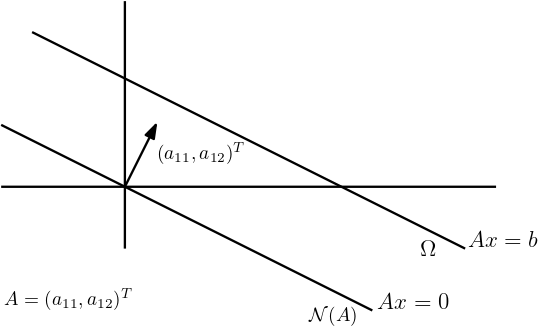
\includegraphics[width=0.60\textwidth]{nucleoA_paralelo_Omega}
	\caption{ Núcleo de uma matriz. \\ Fonte: \textcite{Ana1994} \label{fig:nucleoA_paralelo_Omega}}
\end{figure}


Como $\posto (A)=m$, as $m$ linhas de $A$ formam um conjunto de vetores linearmente independentes que geram o subespaço chamado imagem de $A^{T}$ de dimensão $m$, que é denotado por $Im(A^{T})$. Dessa forma, como é possível observar na \Cref{fig:nucleoA_paralelo_Omega}, as linhas de $A$ são ortogonais ao $\mathcal{N}(A)$, ou, em outras palavras, $\mathcal{N}(A)$ é o complemento ortogonal de $Im(A^{T})$. Vamos demonstrar este resultado. 

\begin{prop} \label{prop:complemento_ortogonal_nucleo}
Seja $A \in \RR^{m\times n}$. $\mathcal{N}(A) = Im(A^{T})^{\bot}$.
\end{prop}
\begin{proof}
Um vetor $v \in \mathcal{N}(A)$ se, e somente se, $Av=0$. Mas isso ocorre se, e somente se, $Av$ é ortogonal a todo vetor $u\in \RR^{m}$, isto é, $u^{T}Av=0$, para todo $u \in \RR^{m}$. Assim, $(u^{T}Av)^{T} = 0^{T}$ implica que $v^{T}(A^{T}u) = 0$. Agora, variando $u \in \RR^{m}$, temos que $A^{T}u$ fornece o conjunto $Im(A^{T})$ e desse modo, $v^{T}(A^{T}v) = 0$, para todo $u \in \RR^{m}$, se, e somente se, $v \in Im(A^{T})^{\bot}$. Portanto, $v\in \mathcal{N}(A)$ se, e somente se, $v\in Im(A^{T})^{\bot}$.
\end{proof}

Assim, $\mathcal{N}(A)$ e $Im(A^{T})$ são subespaços vetoriais ortogonais e verificam
\[ \label{eq:nucleo_imagem_subespacos_geram_Rn} \mathcal{N}(A) \cap Im(A^{T}) = \{ 0 \} \quad \text{e} \quad \RR^{n} = \mathcal{N}(A) \oplus Im(A^{T}) .\]
\begin{obs} 
A demonstração de \eqref{eq:nucleo_imagem_subespacos_geram_Rn} está disponível em \textcite{Elon2014}.
\end{obs}

A partir disso, se $d \in \mathcal{N}(A)$ e $\tilde{x}$ é uma solução da restrição \eqref{eq:restricao_de_igualdade}, então $x\coloneqq  \tilde{x} + \alpha d$ também é solução de \eqref{eq:restricao_de_igualdade}, pois
\[
A(\tilde{x} + \alpha d) = A\tilde{x}
 + \alpha Ad = A\tilde{x} = b
\]
 e portanto, qualquer $d \in \mathcal{N}(A)$ é uma direção no espaço na qual podemos nos deslocar a partir de uma solução factível sem correr o risco de abandonar a região de factibilidade. 

A recíproca também é verdadeira, pois se a partir de uma solução factível $\tilde{x}$, andando numa direção $d \in \RR^{n}$ obtemos
\[
x=\tilde{x} + \alpha d \quad \text{e} \quad Ax=b ,
\]
então $A(\tilde{x} + \alpha d) = b$ implica em $Ad = 0$ e, portanto, $d \in \mathcal{N}(A)$. Dessa forma, concluímos que $\mathcal{N}(A)$ é o conjunto de direções factíveis em $\Omega$.

A partir disso, é possível construir uma parametrização que caracterize o conjunto factível. Se $\{ z_{1}, z_{2}, \ldots , z_{n-m} \}$ é uma base de $\mathcal{N}(A)$ e $Z$ a matriz de dimensão $n\times (n-m)$ cujas colunas são os vetores $z_{i}$, então para todo $d \in \mathcal{N}(A)$, existe $\boldsymbol{\gamma} \in \RR^{n-m}$ tal que $d=Z\boldsymbol{\gamma}$, ou seja, $d$ é escrito como combinação linear dos vetores da base do núcleo de A. Assim, se $\tilde{x}$ é uma solução de \eqref{eq:restricao_de_igualdade}, podemos caracterizar o conjunto factível da seguinte forma
\[ \label{parametrizacao_de_S}
\Omega = \{ x \in \RR^{n} \mid x=\tilde{x} + Z\boldsymbol{\gamma} , \ \boldsymbol{\gamma} \in \RR^{n-m} \ \text{e} \ A\tilde{x} =b \} .
\]

\subsubsection{Condições Necessárias de Primeira Ordem} \label{subsection:condicoes_1ordem_igualdade}

Como vimos anteriormente, de modo geral, se um ponto é solução de um problema de otimização então deve satisfazer determinadas propriedades, que são chamadas de condições de otimalidade. Nesta seção abordaremos a condição necessária de primeira ordem para o problema de minimização com restrições de igualdade. Para obter esta condição utilizaremos a parametrização do conjunto factível proposta em \eqref{parametrizacao_de_S}, transferindo as restrições de \eqref{problema_geral_minimizacao_igualdade} para sua função objetivo. Com isso obtemos um novo problema de minimização irrestrita, para o qual as condições necessárias de primeira e segunda ordem já são conhecidas.

Assim sendo, a caracterização de $\Omega$ dada em \eqref{parametrizacao_de_S} permite definir a seguinte função $\varphi : \RR^{n-m} \rightarrow \RR$ dada por
\[ \label{funcao_phi_restricoes_igualdade}
\varphi (\boldsymbol{\gamma}) = f(\tilde{x} + Z\boldsymbol{\gamma}),
\]
e a partir dela podemos considerar o seguinte problema de minimização sem restrições
\[ \label{problema_minimizacao_irrestrita_phi}
\min_{\boldsymbol{\gamma}} \varphi (\boldsymbol{\gamma}) .
\]

Primeiramente, vejamos que os problemas \eqref{problema_geral_minimizacao_igualdade} e \eqref{problema_minimizacao_irrestrita_phi} são equivalentes.

\begin{prop} \label{prop:equivalencia_problema_restricoes_igualdade_irrestrito}
O vetor $\boldsymbol{\gamma}^{*}$ é um minimizador local (global) de $\varphi$ em $\RR^{n-m}$ se, e somente se, $x^{*} \coloneqq  \tilde{x} + Z\boldsymbol{\gamma}^{*}$ é um minimizador local (global) de \eqref{problema_geral_minimizacao_igualdade}.
\end{prop}
\begin{proof}
Seja $\boldsymbol{\gamma}^{*}$ um minimizador local (global) de $\varphi$ em $\RR^{n-m}$. Então,
\[
f(\tilde{x} + Z\boldsymbol{\gamma}^{*} ) = \varphi (\boldsymbol{\gamma}^{*}) \leq \varphi (\boldsymbol{\gamma}) = f(\tilde{x} + Z\boldsymbol{\gamma}) ,
\]
para todo $\boldsymbol{\gamma} \in \RR^{n-m}$. Logo, chamando $x^{*}\coloneqq \tilde{x} + Z\boldsymbol{\gamma}^{*} \in \Omega$, temos
\[
f(x^{*}) \leq f(x),
\]
para todo $x \in \Omega$. Portanto, $x^{*}$ é um minimizador local (global) de \eqref{problema_geral_minimizacao_igualdade}.

Reciprocamente, suponhamos que $x^{*}=\tilde{x} + Z\boldsymbol{\gamma}^{*}$, com $\boldsymbol{\gamma}^{*} \in \RR^{n-m}$, é um minimizador local (global) de \eqref{problema_geral_minimizacao_igualdade}. Então,
\[ \label{eq:1_prop:equivalencia_problema_restricoes_igualdade_irrestrito}
f(\tilde{x} + Z\boldsymbol{\gamma}^{*}) = f(x^{*}) \leq f(x) = f(\tilde{x} + Z\boldsymbol{\gamma})
\]
para todo $x \in \Omega$ e $\boldsymbol{\gamma} \in \RR^{n-m}$. Assim, a definição \eqref{funcao_phi_restricoes_igualdade} da função $\varphi$ e \eqref{eq:1_prop:equivalencia_problema_restricoes_igualdade_irrestrito} implicam em 
\[
\varphi(\boldsymbol{\gamma}^{*}) \leq \varphi(\boldsymbol{\gamma}) , 
\]
para todo $\boldsymbol{\gamma} \in \RR^{n-m}$. Portanto, $\boldsymbol{\gamma}^{*}$ é um minimizador local (global) de $\varphi$ em $\RR^{n-m}$.
\end{proof}

Agora, como \eqref{problema_minimizacao_irrestrita_phi} é um problema de minimização irrestrito, o \Cref{teo:condicao_necessaria_1_ordem} nos diz que a condição necessária de primeira ordem para algum $\boldsymbol{\gamma}^{*} \in \RR^{n-m}$ é
\[ \label{condicao_1_ordem_phi}
\nabla \varphi(\boldsymbol{\gamma}^{*}) = 0.
\]

Por \eqref{funcao_phi_restricoes_igualdade} e definindo a função $g: \RR^{n-m} \rightarrow \RR^{n}$, com $g(\boldsymbol{\gamma}) = \tilde{x} + Z\boldsymbol{\gamma}$, temos que $\varphi(\boldsymbol{\gamma}) = f(g(\boldsymbol{\gamma}))$. Aplicando a regra da cadeia para calcular sua derivada, obtemos
\[
\nabla \varphi (\boldsymbol{\gamma})^{T} = \nabla f(g(\boldsymbol{\gamma})) J_{g}(\boldsymbol{\gamma}) ,
\]
em que $J_{g}(\boldsymbol{\gamma})$ é a matriz Jacobiana de $g$ em $\boldsymbol{\gamma}$. Note que $J_{g}(\boldsymbol{\gamma}) = Z$, portanto
\[
\nabla \varphi(\boldsymbol{\gamma}) = Z^{T}\nabla f(g(\boldsymbol{\gamma})) .
\]

Desse modo, da condição \eqref{condicao_1_ordem_phi}, resulta que
\[
0 = \nabla \varphi (\boldsymbol{\gamma}^{*}) = Z^{T} \nabla f(\tilde{x} + Z\boldsymbol{\gamma}^{*}) = Z^{T} \nabla f(x^{*}).
\]

Portanto, uma condição necessária de primeira ordem para que $x^{*}$ seja minimizador local de \eqref{problema_geral_minimizacao_igualdade} é que
\[ \label{condicao_1_ordem_f}
Z^{T} \nabla f(x^{*}) = 0,
\]
ou seja, que $(z_{i})^{T} \nabla f(x^{*}) =0$, para todo $i=1, \ldots , n-m$. Como $\{ z_{1}, \ldots , z_{n-m} \}$ é uma base de $\mathcal{N}(A)$, tal condição implica que $\nabla f(x^{*})$ seja ortogonal a $\mathcal{N}(A)$. Logo, pelas considerações feitas anteriormente, temos que $\nabla f(x^{*}) \in Im(A^{T})$, em outras palavras, $\nabla f(x^{*})$ deve ser uma combinação linear das linhas de $A$. Portanto, existe $\boldsymbol{\lambda}^{*} \in \RR^{m}$ tal que
\[ \label{condicao_1_ordem_gradiente}
\nabla f(x^{*}) = A^{T} \boldsymbol{\lambda}^{*} .
\] 

Observe que as condições propostas em \eqref{condicao_1_ordem_f} e \eqref{condicao_1_ordem_gradiente} são equivalentes. Com efeito, se \eqref{condicao_1_ordem_f} se verifica, isso implica que $\nabla f(x^{*}) \in \mathcal{N}(A)^{\bot} = Im(A^{T})$ e portanto \eqref{condicao_1_ordem_gradiente} é verdadeiro. Reciprocamente, se \eqref{condicao_1_ordem_gradiente} ocorre, temos que, pela \Cref{prop:complemento_ortogonal_nucleo}, $Z^{T}\nabla f(x^{*}) = Z^{T}(A^{T} \boldsymbol{\lambda}^{*}) = 0$.

Em vista disso, se $x^{*}$ é um minimizador local de \eqref{problema_geral_minimizacao_igualdade}, então, por \eqref{condicao_1_ordem_gradiente}, existe $\boldsymbol{\lambda}^{*} \in \RR^{m}$ tal que $(x^{*}, \boldsymbol{\lambda}^{*})$ é solução do seguinte sistema de $(n+m)$ equações
\[ \label{problema_restricoes_igualdade_dual}
\begin{aligned}
& \nabla f(x^{*}) = A^{T} \boldsymbol{\lambda}^{*} \\
& Ax^{*} = b .
\end{aligned}
\]

A solução de \eqref{problema_geral_minimizacao_igualdade} é necessariamente solução de \eqref{problema_restricoes_igualdade_dual}, porém para a recíproca ser verdadeira é necessária a informação de segunda ordem.

O vetor $\boldsymbol{\lambda}^{*} \in \RR^{m}$ é chamado vetor de \emph{multiplicadores de Lagrange} associado a $x^{*}$.

Vejamos a seguir um exemplo em que as condições de otimalidade de primeira ordem nos permitem determinar a expressão geral para uma solução de um problema.

\begin{exem}
Queremos encontrar uma solução do sistema linear $Ax =b$, em que $m<n$, (portanto um sistema linear com infinitas soluções), com a menor norma possível. Podemos descrever matematicamente este problema da seguinte forma
\[\begin{aligned} \label{exem:minimizar_norma}
\min_{x} & \quad \dfrac{1}{2}\Vert x \Vert^{2} \\
\text{s.a} & \quad Ax=b,
\end{aligned} \]
com $x \in \RR^{n}$, $A \in \RR^{m\times n}$, $b\in \RR^{m}$, $m<n$ e $\posto (A)=m$. Com efeito, seja $\tilde{x}$ solução de \eqref{exem:minimizar_norma}. Então, $\tilde{x}$ também minimiza $\Vert x \Vert^{2}$ que por sua vez minimiza $\Vert x \Vert$, pois os problemas são equivalentes. Além disso, veremos que a solução $\tilde{x}$ desse problema pode ser escrita como $\tilde{x} = A^{\dag}b$, em que $A^{\dag} \in \RR^{n\times m}$ e $AA^{\dag} =I$.
\end{exem}
Assim, inicialmente $\tilde{x}$ deve satisfazer a restrição de igualdade, isto é,
\[ \label{exem:minimizar_norma_verifica_restricao}
A\tilde{x} = b .
\]
Além disso, se $\tilde{x}$ é solução então,
\[
\nabla f(\tilde{x}) =A^{T} \tilde{\boldsymbol{\lambda}},
\]
e como $\nabla f(\tilde{x}) = \tilde{x}$, obtemos 
\[ \label{exem:minimizar_norma_gradiente}
\tilde{x} = A^{T} \tilde{\boldsymbol{\lambda}} .
\]
Substituindo \eqref{exem:minimizar_norma_gradiente} em \eqref{exem:minimizar_norma_verifica_restricao}, temos
\[
AA^{T} \tilde{\boldsymbol{\lambda}} = b,
\]
e como por hipótese $A$ é posto completo, temos que $AA^{T}$ é não singular. Desse modo,
\[
(AA^{T})^{-1} AA^{T} \tilde{\boldsymbol{\lambda}} = (AA^{T})^{-1} b,
\]
o que implica em 
\[ \label{exem:minimizar_norma_lambdatil}
\tilde{\boldsymbol{\lambda}} = (AA^{T})^{-1} b.
\]
Agora, substituindo \eqref{exem:minimizar_norma_lambdatil} em \eqref{exem:minimizar_norma_gradiente}, concluímos que
\[
\tilde{x} = A^{T}(AA^{T})^{-1}b = A^{\dag} b,
\]
em que $A^{\dag} = A^{T}(AA^{T})^{-1} \in \RR^{n\times m}$ e $AA^{\dag} = AA^{T}(AA^{T})^{-1} = I$.

\begin{obs}
A matriz $A^{\dag}$ é também chamada de \emph{pseudo-inversa} de Moore-Penrose. Para mais informações consulte \textcite[p.423]{meyer2000matrix}.
\end{obs}


\subsubsection{Condições Necessárias e Suficientes de Segunda Ordem} \label{subsubsection:condicao_2ordem_igualdade}

A condição necessária de segunda ordem para uma solução $x^{*}$ do problema \eqref{problema_minimizacao_irrestrita_phi} é dada pelo \Cref{teo:condicao_necessaria_2_ordem} e toma a seguinte forma
\[ \label{hessiana_phi}
\nabla^{2} \varphi (\boldsymbol{\gamma}^{*}) \succcurlyeq 0.
\]

Derivando $\nabla \varphi (\boldsymbol{\gamma}) = Z^{T}\nabla f(\tilde{x} + Z\boldsymbol{\gamma})$ através da regra da cadeia, obtemos
\[
\nabla^{2} \varphi(\boldsymbol{\gamma}) = Z^{T} \nabla^{2} f(\tilde{x} + Z\boldsymbol{\gamma})Z .
\]
Assim, por \eqref{hessiana_phi} temos que a condição necessária de segunda ordem para que $x^{*}$ seja minimizador local de \eqref{problema_geral_minimizacao_igualdade} é
\[
Z^{T} \nabla^{2} f(x^{*})Z \succcurlyeq 0.
\]

Ademais, observe que $Z^{T}\nabla^{2} f(x^{*})Z$ é uma matriz de ordem $(n-m)\times (n-m)$, e o fato de ser semidefinida positiva significa que
\[
y^{T}\nabla^{2} f(x^{*})y \geq 0 \ \text{para todo} \ y \in \mathcal{N}(A) .
\]
Isso significa que $\nabla^{2} f(x^{*})$ é semidefinida positiva para todo $y\in \mathcal{N}(A)$.

Analogamente, a partir das condições suficientes para o problema \eqref{problema_minimizacao_irrestrita_phi}, podemos determinar as seguintes condições suficientes de segunda ordem para \eqref{problema_geral_minimizacao_igualdade}.

\begin{teo}(\textbf{Condição suficiente de segunda ordem}) \label{teo:condicao_suficiente_2ordem_igualdade}
Se $x^{*} \in \RR^{n}$ verifica $Ax^{*}=b$ e 
\begin{enumerate}
	\item[(i)] $Z^{T}\nabla f(x^{*}) =0$,
	\item[(ii)] $Z^{T}\nabla^{2} f(x^{*})Z \succ 0$ (definida positiva),
\end{enumerate}	
então $x^{*}$ é um minimizador local de \eqref{problema_geral_minimizacao_igualdade}.
\end{teo}

\begin{prop}
Seja $f: \RR^{n} \rightarrow \RR$, $f \in \mathcal{C}^{2}$. Seja $\tilde{x} \in \RR^{n}$ tal que $A\tilde{x} = b$ ($A\in \RR^{m\times n}$, $b\in \RR^{m}$) e tal que existe $\boldsymbol{\lambda} \in \RR^{m}$ com $\nabla f(\tilde{x}) = A^{T}\boldsymbol{\lambda}$ e $\nabla^{2} f(\tilde{x})$ definida positiva. Então $\tilde{x}$ é um minimizador local de $f$ sujeita a $Ax=b$.
\end{prop}
\begin{proof}
Para provar que $\tilde{x}$ é minimizador local de $f$ vamos verificar se ele satisfaz as condições suficientes de segunda ordem. Por hipótese temos que $\tilde{x} \in \RR^{n}$ satisfaz a restrição $A\tilde{x} = b$. Por conseguinte, existe $\boldsymbol{\lambda} \in \RR^{m}$ tal que $\nabla f(\tilde{x}) = A^{T}\boldsymbol{\lambda}$. Assim, seja Z a matriz cujas colunas são os vetores de uma base do $\mathcal{N}(A)$. Sabemos que as linhas de $A$ são ortogonais a $\mathcal{N}(A)$ e portanto,
\[
Z^{T}\nabla f(\tilde{x}) = Z^{T}A^{T}\boldsymbol{\lambda} = 0.
\]
Além disso, como $\nabla^{2} f(\tilde{x})$ é definida positiva e a matriz $Z$ é posto completo, temos que 
\[
Z^{T}\nabla^{2} f(\tilde{x}) Z \succ 0.
\]
Portanto, $\tilde{x}$ é minimizador local de $f$.
\end{proof}

Vejamos um exemplo em que as condições suficientes nos permitem determinar uma solução para o problema de minimizar uma função quadrática sujeita a restrições de igualdade.

\begin{exem}
Considere o problema
\[ \begin{aligned} \label{exem:minimizar_quadratica_problema}
\min_{x} & \quad \dfrac{1}{2}x^{T}Qx + p^{T}x + q \\
\text{s.a} & \quad Ax = b,
\end{aligned} \]
em que $Q \in \RR^{n\times n}$ é simétrica, $ x,p \in \RR^{n}$, $q \in \RR$, $A \in \RR^{m\times n}$ e $b \in \RR^{m}$. Seja $Z$ uma base do $\mathcal{N}(A)$ e suponha que $Z^{T}QZ$ é definida positiva. Seja $x^{0}$ tal que $Ax^{0}=b$. Então a solução $\tilde{x}$ é dada por
\[ \label{exem:minimizar_quadratica_solucao}
\tilde{x} = x^{0} - Z(Z^{T}QZ)^{-1} Z^{T}(Qx^{0} + p).
\]
\end{exem}
Para provar que \eqref{exem:minimizar_quadratica_solucao} é solução é preciso verificar se $\tilde{x}$ cumpre as condições suficientes de segunda ordem. Para tanto, devemos ter:
\begin{enumerate}
	\item[(i)] $\tilde{x}$ cumpre a restrição de igualdade. De fato,
	\[ \begin{aligned}
	A\tilde{x} = & A(x^{0} - Z(Z^{T}QZ)^{-1} Z^{T}(Qx^{0} + p)) \\
	= & Ax^{0} - AZ(Z^{T}QZ)^{-1} Z^{T}(Qx^{0} + p) \\
	= & b,
	\end{aligned} \]
	pois $AZ=0$ pelo fato de cada coluna de $Z$ pertencer ao $\mathcal{N}(A)$ e portanto, serem ortogonais as linhas de $A$.

	\item[(ii)] É preciso verificar se $Z^{T}\nabla f(\tilde{x}) = 0$. Como $\nabla f(\tilde{x}) = Q\tilde{x} + p$, temos que
	\[ \begin{aligned}
	Z^{T}(Q\tilde{x} +p) =& Z^{T} Q (x^{0} - Z(Z^{T}QZ)^{-1}Z^{T}(Qx^{0} +p)) + Z^{T}p \\
	=& Z^{T} Qx^{0} - Z^{T}QZ(Z^{T}QZ)^{-1}Z^{T}(Qx^{0} +p) + Z^{T}p \\
	=& Z^{T} Qx^{0} - Z^{T} Qx^{0} - Z^{T} p + Z^{T} p \\
	=& 0.
	\end{aligned} \]

	\item[(iii)] Por fim, $Z^{T}\nabla^{2} f(\tilde{x})Z$ deve ser definida positiva. Assim, como $\nabla^{2} f(\tilde{x}) = Q$, temos que 
	\[
	Z^{T}QZ \succ 0.
	\]
\end{enumerate}
Portanto, $\tilde{x}$ é solução do problema \eqref{exem:minimizar_quadratica_problema}.

\begin{obs}
Veremos mais a frente que no caso em que $Q$ é uma matriz semidefinida positiva, os problemas quadráticos são convexos.
\end{obs}


%-------------------------------------------------------------------------------------------------------------------
\subsection{Minimização com Restrições Lineares de Desigualdade} \label{section:restricoes_desigualdade}

Vamos considerar agora problemas da forma
\[ \label{problema_geral_minimizacao_desigualdade}
\begin{aligned}
\min_{x} & \quad f(x) \\
\text{s.a} & \quad Wx \leq c,
\end{aligned}
\]
em que $x \in \RR^{n}$ e $W \in \RR^{m\times n}$. Como na seção anterior, estamos interessados nesse primeiro momento em analisar a região de factibilidade e determinar as direções factíveis, que são aquelas em que há espaço para se movimentar dentro da região $\Omega$. 

Denotando cada linha da matriz $W$ da forma $w_{i}^{T} = (w_{i1} , w_{i2} , \ldots , w_{in})$, podemos caracterizar o conjunto factível da seguinte forma
\[
\Omega = \{ x\in \RR^{n} \mid w_{i}^{T}x \leq c_{i} \ \text{para todo} \ i = 1,2, \ldots , m \} .
\]

Cada uma das $m$ desigualdades $w_{i}^{T}x \leq c_{i}$ define em $\RR^{n}$ um \emph{semiespaço}. O hiperplano divisor é dado por $\Hset (w_{i}, c_{i}) = \{ x \mid w_{i}^{T}x = c_{i} \}$ e o semiespaço definido é aquele que está do lado contrário à direção apontada pelo vetor $w_{i}$. Desta forma, a região $\Omega$ consiste na intersecção dos $m$ semiespaços. Este tipo de conjunto de $\RR^{n}$ é chamado \emph{poliedro} ou conjunto \emph{poliedral}. Vamos definir formalmente este conceito.


\begin{defi} \label{defi:conjunto_poliedral}
Um \emph{poliedro} ou um conjunto \emph{poliedral} $\mathcal{P} \subset \RR^{n}$ é definido como o conjunto de soluções de um sistema finito de equações e inequações lineares:
\[
\mathcal{P} = \{ x\in \RR^{n} \mid Ax=b, \ Wx \leq c \} ,
\] 
em que $A\in \RR^{m\times n}$, $W\in \RR^{p\times n}$, $b\in \RR^{m}$ e $c\in \RR^{p}$. Neste contexto, dizemos que $h:\RR^{n} \rightarrow \RR^{m}$, dada por $h(x) = Ax-b$, e $g:\RR^{n} \rightarrow \RR^{p}$, dada por $g(x)=Wx-c$, são funções \emph{afim}.
\end{defi}

A \Cref{fig:regiao_factivel_poliedro} representa um poliedro em $\RR^{2}$.

\begin{figure}[!ht] 
	\centering
	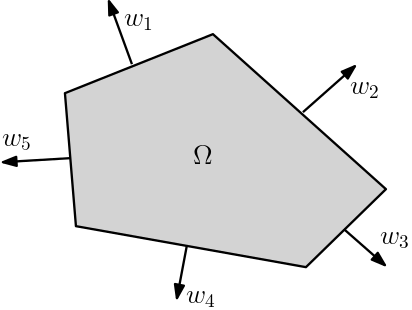
\includegraphics[width=0.45\textwidth]{conjunto_factivel_poliedral}
	\caption{Conjunto factível poliedral. \\ Fonte: \textcite{Ana1994} \label{fig:regiao_factivel_poliedro}}
\end{figure}

Um conceito fundamental para formular as condições de otimalidade para o problema \eqref{problema_geral_minimizacao_desigualdade} e que fornece uma grande quantidade de informações é o de \emph{restrição ativa}. Portanto, consideramos, no que segue, que $\Omega$ é o conjunto factível deste problema.

\begin{defi}
Dado $\xbar \in \Omega$, dizemos que a restrição de desigualdade $w_{i}^{T}\bar{x} \leq c_{i}$ que corresponde ao índice $i\in \{ 1,2, \ldots , m\}$ é \emph{ativa} no ponto $\xbar$ quando $w_{i}^{T}\bar{x} = c_{i}$. Caso $w_{i}^{T}\bar{x} < c_{i}$ dizemos que a restrição é \emph{inativa} em $\xbar$. O conjunto dos índices das restrições de desigualdade ativas no ponto $\xbar \in \Omega$ é denotado por
\[
\mathcal{I} (\xbar) = \{ i = 1,2, \ldots , m \mid w_{i}^{T}\bar{x} = c_{i} \} .
\]
\end{defi} 

%\begin{obs}
%Por convenção, qualquer restrição de igualdade é considerada ativa em todo ponto factível.
%\end{obs}

A cada $x\in \Omega$ podemos associar um número $r(x)$, com $0\leq r(x) \leq m$, que representa a quantidade de restrições ativas em $x$. Assim, na \Cref{fig:restricoes_ativas} temos que $r(x^{1}) = 1$, $r(x^{2}) = 2$, $r(x^{3}) = 1$, $r(x^{4}) = 0$ e $r(x^{5}) = 2$.

\begin{figure}[!ht] 
	\centering
	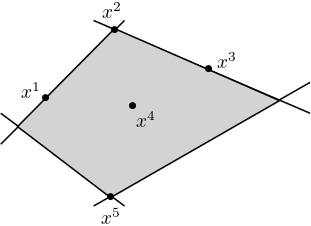
\includegraphics[width=0.45\textwidth]{restricoes_ativas}
	\caption{Restrições ativas e inativas. \label{fig:restricoes_ativas}}
\end{figure}

Ademais, o conjunto das direções factíveis a partir de $x$ depende das restrições ativas nesse ponto, pois são elas que restringem o domínio de factibilidade na vizinhança de $x$, enquanto que as restrições inativas não possuem influência na vizinhança de $x$.
O \Cref{teo:direcoes_factiveis_restricao_desigualdade} nos fornece uma caracterização das direções factíveis em $x$.

\begin{teo} \label{teo:direcoes_factiveis_restricao_desigualdade}
Considere $x\in \Omega$ tal que $r(x) = p$ com $0<p \leq m$. Um vetor $d \in \RR^{n}$ é uma direção factível a partir de $x$ se, e somente se, $w_{i}^{T}d \leq 0$ para todo $i \in \mathcal{I} (x)$.
\end{teo}
\begin{proof}
Suponhamos que $d\in \RR^{n}$ é uma direção factível em $x$. Então existe $\tilde{\alpha} >0$ tal que $x+\alpha d \in \Omega$ para todo $\alpha \in (0, \tilde{\alpha} ]$, o que ocorre se, e somente se, $W(x+\alpha d) \leq c$, ou seja, $w_{i}^{T}(x+\alpha d) \leq c_{i}$, para todo $i \in \mathcal{M} \coloneqq \{ 1,2, \ldots ,m \}$. 
Em particular, se $i\in \mathcal{I} (x)$ temos que
\[
w_{i}^{T}(x+\alpha d) = c_{i} + \alpha w_{i}^{T}d \leq c_{i},
\]
e consequentemente, temos
\[
w_{i}^{T}d \leq 0.
\]

Reciprocamente, seja $d\in \RR^{n}$ e suponhamos que $w_{i}^{T}d \leq 0$ para todo $i \in \mathcal{I} (x)$. Assim, se $i \in \mathcal{I} (x)$, temos que $w_{i}^{T} x = c_{i}$, implicando que, para qualquer $\alpha >0$, $w_{i}^{T}(x+\alpha d) \leq c_{i}$.
Por outro lado, se $i \notin \mathcal{I}(x)$, temos que $w_{i}^{T} x < c_{i}$. Neste caso, é preciso analisar duas situações:
\begin{enumerate}
	\item[(i)] Se $w_{i}^{T}d \leq 0$, então $w_{i}^{T}(x + \alpha d) \leq c_{i}$, para qualquer $\alpha >0$             ;

	\item[(ii)]Se $w_{i}^{T}d >0$ podemos encontrar $\alpha_{i} >0$ de modo que $w_{i}^{T}x + w_{i}^{T}(\alpha_{i} d) = c_{i}$. Considere que como $w_{i}^{T}x < c_{i}$ existe $\beta >0$, tal que $w_{i}^{T}x + \beta_{i} = c_{i}$. Desse modo, temos que escolher $\alpha_{i}$ tal que $\beta_{i} = \alpha_{i} w_{i}^{T} d$, isto é,
	\[
	w_{i}^{T}x + \alpha_{i} w_{i}^{T}d = c_{i} ,
	\]
	para todo $i \notin \mathcal{I}(x)$. Podemos fazer isso resolvendo a equação anterior para $\alpha_{i}$, encontrando
	\[ \label{eq:1_teo_direcoes_factiveis_restricao_desigualdade}
	\alpha_{i} = \dfrac{c_{i} - w_{i}^{T}x}{w_{i}^{T}d}.
	\]
	Assim, se tomarmos o mínimo de \eqref{eq:1_teo_direcoes_factiveis_restricao_desigualdade}, para todo $i \in \mathcal{M} \backslash \mathcal{I}(x)$, isto é, se definirmos
	\[ \label{eq:2_teo_direcoes_factiveis_restricao_desigualdade}
	\tilde{\alpha} = \min_{i \in \mathcal{M} \backslash \mathcal{I}(x) } \left( \dfrac{c_{i} - w_{i}^{T}x}{w_{i}^{T}d} \right) ,
	\]
	teremos que $w_{i}^{T}(x + \alpha d) \leq c_{i}$ para todo $i \in \mathcal{M}$ e $\alpha \in (0,\tilde{\alpha} ]$. 
\end{enumerate}	
Portanto, de (i) e (ii), $d$ será uma direção factível a partir de $x$.
\end{proof}

A demonstração do \Cref{teo:direcoes_factiveis_restricao_desigualdade} nos dá, na equação \eqref{eq:2_teo_direcoes_factiveis_restricao_desigualdade}, o quanto podemos andar em uma direção factível $d$ a partir de $x \in \Omega$ e ainda continuarmos sobre o conjunto factível.


\subsubsection{Condições Necessárias de Primeira Ordem}

No intuito de determinar as condições de otimalidade no caso de problemas com restrições de desigualdade, acabamos de desenvolver a noção de direções factíveis para avaliar a estrutura do conjunto factível na vizinhança de uma solução. Agora, é necessário definir o conceito de direção de descida.

\begin{defi} \label{defi:direcao_de_descida}
Dizemos que $d\in \RR^{n}$ é uma \emph{direção de descida} de $f:\RR^{n} \rightarrow \RR$ no ponto $\xbar \in \RR^{n}$, se existe $\varepsilon >0$ tal que
\[
f(\xbar + td) <f(\xbar)
\]
para todo $t \in (0,\varepsilon ]$.
\end{defi}
Denotamos por $\mathcal{D}_{f}(\xbar)$ o conjunto de todas as direções de descida da função $f$ no ponto $\xbar$.


\begin{lema} \label{lema:direcao_de_descida}
Seja $f:\RR^{n} \rightarrow \RR$ uma função diferenciável no ponto $\xbar \in \RR^{n}$. Então
\begin{enumerate}
	\item[(i)] Para todo $d \in \mathcal{D}_{f}(\xbar)$, tem-se que $\nabla f(\xbar)^{T}d \leq 0$.

	\item[(ii)] Se $d\in \RR^{n}$ satisfaz $\nabla f(\xbar)^{T}d < 0$, tem-se que $d \in \mathcal{D}_{f}(\xbar)$.
\end{enumerate}	
\end{lema}
\begin{proof}
Seja $d \in \mathcal{D}_{f}(\xbar)$. Assim, para todo $t>0$ suficientemente pequeno, 
\[ \label{eq:1_lema_direcao_de_descida}
f(\xbar + td) < f(\xbar).
\]
Pelo \Cref{fato:Taylor_primeira_ordem}, temos
\[ \label{eq:2_lema_direcao_de_descida}
f(\xbar + td) - f(\xbar) = t\nabla f(\xbar)^{T} d + o(t),
\] 
com $\lim_{t\rightarrow 0} \dfrac{o(t)}{t} =0$, e de \eqref{eq:1_lema_direcao_de_descida} e \eqref{eq:2_lema_direcao_de_descida}, obtemos
\[ \label{eq:3_lema_direcao_de_descida}
t\nabla f(\xbar)^{T}d + o(t) < 0.
\]
Dividindo ambos os lados da desigualdade \eqref{eq:3_lema_direcao_de_descida} por $t>0$ e passando o limite quando $t \rightarrow 0^{+}$, obtemos
\[
\nabla f(\xbar)^{T}d \leq 0,
\]
provando o item $(i)$.

Suponhamos agora que $\nabla f(\xbar)^{T}d <0$. Aplicando o \Cref{fato:Taylor_primeira_ordem}, podemos escrever
\[
f(\xbar + td) - f(\xbar) = t\left( \nabla f(\xbar)^{T}d + \dfrac{o(t)}{t} \right) .
\]
Em particular, para todo $t>0$ suficientemente pequeno, temos
\[
\nabla f(\xbar)^{T}d + \dfrac{o(t)}{t} \leq \dfrac{1}{2} \nabla f(\xbar)^{T}d <0,
\]
o que implica em
\[
f(\xbar + td) - f(\xbar) <0.
\]
Portanto, $d \in \mathcal{D}_{f}(\xbar)$.
\end{proof}

Assim, a partir de um ponto $\xbar \in \Omega$, estamos interessados em saber se existem direções de descida factíveis, isto é, direções factíveis tais que
\[ \label{eq:caracterizacao_direcao_descida}
\nabla f(\xbar)^{T}d < 0,
\]
pois se existe uma direção $d$ que satisfaz \eqref{eq:caracterizacao_direcao_descida}, decorre do \Cref{lema:direcao_de_descida} e da \Cref{defi:direcao_de_descida} que $\xbar$ não é minimizador local do problema \eqref{problema_geral_minimizacao_desigualdade}.

\begin{obs}
Novamente, a análise dependerá das restrição ativas em $\xbar$. Se $r(\xbar) =0$, o ponto está no interior de $\Omega$ e as condições necessárias e suficientes são as mesmas do caso em que o problema é irrestrito.
\end{obs}

Agora, já possuímos os ferramentais necessários para determinar a condição necessária de primeira ordem a ser satisfeita por uma solução do problema \eqref{problema_geral_minimizacao_desigualdade}.



\begin{teo}(\textbf{Condição necessária de primeira ordem}) \label{teo:condicao_necessaria_1ordem_restricao_desigualdade}
Consideremos o problema \eqref{problema_geral_minimizacao_desigualdade} com $f \in \mathcal{C}^{1}$ e $x^{*} \in \Omega$ tal que $1 \leq r(x^{*}) \leq n$. Seja $\mathcal{I} \subset \mathcal{M}$, $\mathcal{I} = \{ i_{1}, i_{2}, \ldots , i_{r(x^{*})} \}$ tal que $w_{i}^{T}x = c_{i}$ se, e somente se, $i\in \mathcal{I}$. Seja $W_{\mathcal{I}} \in \RR^{r(x^{*})\times n}$ a submatriz de $W$ cujas linhas são as que tem índices em $\mathcal{I}$ e 
\[
c_{\mathcal{I}} = \begin{bmatrix*} c_{i_{1}} \\ c_{i_{2}} \\ \vdots \\ c_{i_{r(x^{*})}} \end{bmatrix*} .
\]
Supomos que $\posto (W_{\mathcal{I}}) = r(x^{*})$.

Se $x^{*}$ é minimizador local de \eqref{problema_geral_minimizacao_desigualdade}, então existe $\boldsymbol{\mu} \in \RR^{r(x^{*})}$ tal que 
\[ \label{eq:condicao_necessaria_1ordem_restricao_desigualdade_somatorio}
\nabla f(x^{*}) + \sum_{k=1}^{r(x^{*})} \mu_{k} w_{i_{k}} = 0 \quad \text{e} \quad \mu_{k} \geq 0, \ 1\leq k\leq r(x^{*}),
\]
ou, equivalentemente
\[ \label{eq:condicao_necessaria_1ordem_restricao_desigualdade}
\nabla f(x^{*}) + W_{\mathcal{I}}^{T} \boldsymbol{\mu} =0, \quad \boldsymbol{\mu} \in \RR^{r(x^{*})}
\]
e
\[
\mu_{k} \geq 0, \ 1\leq k\leq r(x^{*}).
\]
\end{teo}
\begin{proof}
Suponhamos, por contradição, que \eqref{eq:condicao_necessaria_1ordem_restricao_desigualdade} não ocorre. Isso pode acontecer por dois motivos:
\begin{enumerate}
\item[(i)] $\nabla f(x^{*}) + W_{\mathcal{I}}^{T} \boldsymbol{\mu} \neq 0 \ \text{para todo} \ \boldsymbol{\mu} \in \RR^{r(x^{*})}$.

Assim, temos que $\nabla f(x^{*})$ não pode ser escrito como combinação linear das linhas de $W_{\mathcal{I}}$. Em outras palavras, $x^{*}$ não é minimizador local do seguinte problema
\[ \label{eq:1_condicao_necessaria_1ordem_restricao_desigualdade}
\begin{aligned}
\min_{x} & \quad f(x) \\
\text{s.a} & \quad W_{\mathcal{I}}x=c_{\mathcal{I}} ,
\end{aligned}
\]
pois $x^{*}$ não satisfaz a condição necessária de primeira ordem para o problema \eqref{eq:1_condicao_necessaria_1ordem_restricao_desigualdade} proposta em \eqref{condicao_1_ordem_gradiente} na \Cref{subsection:condicoes_1ordem_igualdade}. Logo, $x^{*}$ não pode ser minimizador local do problema \eqref{problema_geral_minimizacao_desigualdade}, o que é uma contradição.

\item[(ii)] $\nabla f(x^{*}) + W_{\mathcal{I}}^{T} \boldsymbol{\mu} = 0$, mas existe $j$ tal que $\mu_{j} <0$.

Primeiramente, se $r(x^{*}) = 1$ temos $\mathcal{I} = \{ i_{1} \}$ e então, 
\[
\nabla f(x^{*}) + \mu_{1} w_{i_{1}} =0 ,
\]
com $\mu_{1} <0$, ou equivalentemente, 
\[
\nabla f(x^{*}) = - \mu_{1} w_{i_{1}} ,
\]
com $\mu_{1} <0$. Assim, tomando $d=-\nabla f(x^{*}) = \mu_{1} w_{i_{1}}$, com $\mu_{1} <0$, temos que $d$ é uma direção de descida, pois
\[
\nabla f(x^{*})^{T}d = -\nabla f(x^{*})^{T} \nabla f(x^{*}) = -\Vert \nabla f(x^{*}) \Vert^{2} <0,
\]
e além disso, $d$ é uma direção factível, pois
\[
w_{i_{1}}^{T}d = \mu_{1} w_{i_{1}}^{T}w_{i_{1}} = \mu_{1} \Vert w_{i_{1}} \Vert^{2} < 0,
\]
devido o fato de $\mu_{1} <0$. Desse modo, $d$ é uma direção de descida factível no ponto $x^{*}$, e portanto $x^{*}$ não pode ser minimizador local de \eqref{problema_geral_minimizacao_desigualdade}, contradizendo a hipótese.

Agora, considere o caso em que $2\leq r(x^{*}) \leq n$. Vamos denotar por $\tilde{W_{\mathcal{I}}}$ a matriz obtida retirando a linha $w_{i_{j}}$ que corresponde ao multiplicador $\mu_{j} >0$. Tomando $d=\proj_{\mathcal{N}(\tilde{W_{\mathcal{I}}})} (-\nabla f(x^{*}))$, temos que
\[
(-\nabla f(x^{*}) -d)^{T}d =0,
\]
pois eles são ortogonais (veja \Cref{fig:projecao_gradiente_sobre_nucleoA}), o que implica em
\[ \label{eq:2_condicao_necessaria_1ordem_restricao_desigualdade}
\nabla f(x^{*})^{T}d = -d^{T}d = -\Vert d \Vert^{2} <0.
\]
\begin{figure}[!ht] 
	\centering
	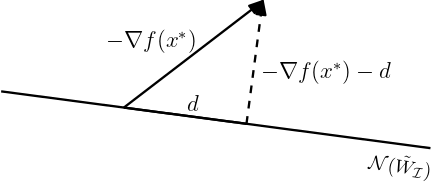
\includegraphics[width=0.55\textwidth]{projecao_gradiente_sobre_nucleoW}
	\caption{Projeção de $-\nabla f(x)$ sobre o $\mathcal{N}(\tilde{W_{\mathcal{I}}})$. \\ Fonte: \textcite{Ana1994}. \label{fig:projecao_gradiente_sobre_nucleoA}}
\end{figure}
Logo, $d$ é uma direção de descida. Além disso, $d$ é uma direção factível. Com efeito, por \eqref{eq:condicao_necessaria_1ordem_restricao_desigualdade_somatorio}, temos que
\[
\nabla f(x^{*}) + \mu_{1} w_{i_{1}} + \mu_{2} w_{i_{2}} + \ldots + \mu_{j} w_{i_{j}} + \ldots + \mu_{r(x^{*})} w_{i_{r(x^{*})}} =0
\]
e, como tomamos $d \in \mathcal{N}(\tilde{W_{\mathcal{I}}})$ temos que
\[ \label{eq:3_condicao_necessaria_1ordem_restricao_desigualdade}
w_{i_{k}}^{T}d =0, 
\]
para todo $k \neq j$. Então,
\[
\nabla f(x^{*})^{T}d + \mu_{j} w_{i_{j}}^{T} d =0,
\]
e reescrevendo, obtemos
\[
\nabla f(x^{*})^{T}d = -\mu_{j} w_{i_{j}}^{T} d =0.
\]
Agora, utilizando \eqref{eq:2_condicao_necessaria_1ordem_restricao_desigualdade} e o fato de $\mu_{j} <0$, obtemos
\[ \label{eq:4_condicao_necessaria_1ordem_restricao_desigualdade}
w_{i_{j}}^{T} d <0.
\]
Assim, de \eqref{eq:3_condicao_necessaria_1ordem_restricao_desigualdade} e \eqref{eq:4_condicao_necessaria_1ordem_restricao_desigualdade}, conluímos que
\[
w_{i_{k}}^{T} d \leq 0
\]
para todo $k$ tal que $1 \leq k \leq r(x^{*})$, ou seja, $d$ é uma direção factível. Portanto, $d$ é uma direção factível e de descida a partir de $x^{*}$, o que contradiz contradizendo o fato de $x^{*}$ ser minimizador local de \eqref{problema_geral_minimizacao_desigualdade}.
\end{enumerate}
\end{proof}


%\begin{teo}(\textbf{Condição necessária de primeira ordem}) \label{teo:condicao_necessaria_1ordem_restricao_desigualdade}
%Consideremos o problema \eqref{problema_geral_minimizacao_desigualdade} com $f \in \mathcal{C}^{1}$ e $x^{*} \in \Omega$ tal que $1 \leq r(x^{*}) \leq n$. Seja $\mathcal{I} \subset \mathcal{M}$, $\mathcal{I} = \{ i_{1}, i_{2}, \ldots , i_{r(x^{*})} \}$ tal que $w_{i}^{T}x = c_{i}$ se, e somente se, $i\in \mathcal{I}$. Seja $W_{\mathcal{I}} \in \RR^{r(x^{*})\times n}$ a submatriz de $W$ cujas linhas são as que tem índices em $\mathcal{I}$ e 
%\[
%c_{\mathcal{I}} = \begin{bmatrix*} c_{i_{1}} \\ c_{i_{2}} \\ \vdots \\ c_{i_{r(x^{*})}} \end{bmatrix*} .
%\]
%Supomos que $\posto (W_{\mathcal{I}}) = r(x^{*})$.

%Se $x^{*}$ é minimizador local de \eqref{problema_geral_minimizacao_desigualdade}, então existe $\boldsymbol{\mu} \in \RR^{r(x^{*})}$ tal que 
%\[
%\nabla f(x^{*}) = \sum_{k=1}^{r(x^{*})} \mu_{k} w_{i_{k}} \quad \text{e} \quad \mu_{k} \leq 0, \ 1\leq k\leq r(x^{*}),
%\]
%ou, equivalentemente
%\[ \label{eq:condicao_necessaria_1ordem_restricao_desigualdade}
%\nabla f(x^{*}) = W_{\mathcal{I}}^{T} \boldsymbol{\mu}, \quad \boldsymbol{\mu} \in \RR^{r(x^{*})}
%\]
%e
%\[
%\mu_{k} \leq 0, \ 1\leq k\leq r(x^{*}).
%\]
%\end{teo}
%\begin{proof}
%Suponhamos que \eqref{eq:condicao_necessaria_1ordem_restricao_desigualdade} não ocorre. Isso pode acontecer por dois motivos:
%\begin{enumerate}
%\item[(i)] $\nabla f(x^{*}) \neq W_{\mathcal{I}}^{T} \boldsymbol{\mu} \ \text{para todo} \ \boldsymbol{\mu} \in \RR^{r(x^{*})}$.

%Em outras palavras, temos que $\nabla f(x^{*})$ não pode ser escrito como combinação linear das linhas de $W_{\mathcal{I}}$. Assim, $x^{*}$ não é minimizador local do problema com restrições de igualdade definido por 
%\[ \label{eq:1_condicao_necessaria_1ordem_restricao_desigualdade}
%\begin{aligned}
%\min_{x} & \quad f(x) \\
%\text{s.a} & \quad W_{\mathcal{I}}x=c_{\mathcal{I}} ,
%\end{aligned}
%\]
%pois $x^{*}$ não satisfaz a condição necessária de primeira ordem para o problema \eqref{eq:1_condicao_necessaria_1ordem_restricao_desigualdade}. Logo, $x^{*}$ também não pode ser minimizador local do problema \eqref{problema_geral_minimizacao_desigualdade}, o que é uma contradição.

%\item[(ii)] $\nabla f(x^{*}) = W_{\mathcal{I}}^{T} \boldsymbol{\mu}$, mas existe $j$ tal que $\mu_{j} >0$.

%Se $r(x^{*}) = 1$ e $\mathcal{I} = \{ i_{1} \}$, então $\nabla f(x^{*}) = \mu_{1} w_{i_{1}}$ e $\mu_{1} >0$. Tomando $d=-\nabla f(x^{*})$ temos que
%\[
%w_{i_{1}}^{T}d = -\mu_{1} w_{i_{1}}^{T}w_{i_{1}} = -\mu_{1} \Vert w_{i_{1}} \Vert^{2} < 0.
%\]
%Assim, $d$ é uma direção de descida factível no ponto $x^{*}$, e portanto, $x^{*}$ não pode ser minimizador local de \eqref{problema_geral_minimizacao_desigualdade}, contradizendo a hipótese.

%Agora, se $2\leq r(x^{*}) \leq n$, denotamos por $\tilde{W_{\mathcal{I}}}$ a matriz obtida retirando a linha $w_{i_{j}}$ correspondente ao multiplicador $\mu_{j} >0$. Consideramos $d=P_{\mathcal{N}(\tilde{W_{\mathcal{I}}})} (-\nabla f(x^{*}))$, em que $P_{\mathcal{N}(\tilde{W_{\mathcal{I}}})}$ é o operador projeção ortogonal sobre $\mathcal{N}(\tilde{W_{\mathcal{I}}})$. Então, temos que
%\[
%(-\nabla f(x^{*}) -d)^{T}d =0,
%\]
%implicando em
%\[ \label{eq:2_condicao_necessaria_1ordem_restricao_desigualdade}
%\nabla f(x^{*})^{T}d = -d^{T}d = -\Vert d \Vert^{2} <0,
%\]
%e portanto, $d$ é uma direção de descida. Veja \Cref{fig:projecao_gradiente_sobre_nucleoA}.

%\begin{figure}[!ht] 
%	\centering
%	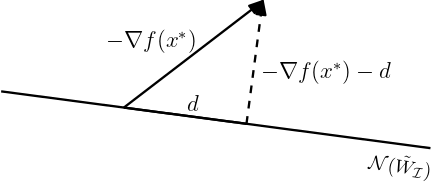
\includegraphics[width=0.55\textwidth]{projecao_gradiente_sobre_nucleoW}
%	\caption{Projeção de $-\nabla f(x)$ sobre o $\mathcal{N}(\tilde{W_{\mathcal{I}}})$. \\ Fonte: \textcite{Ana1994}. \label{fig:projecao_gradiente_sobre_nucleoA}}
%\end{figure}
%Ademais, vejamos que $d$ também é uma direção factível. Com efeito,
%\[
%\nabla f(x^{*}) = \mu_{1} w_{i_{1}} + \mu_{2} w_{i_{2}} + \ldots + \mu_{j} w_{i_{j}} + \ldots + \mu_{r(x^{*})} w_{i_{r(x^{*})}}
%\]
%e, por construção, como tomamos $d \in \mathcal{N}(\tilde{W_{\mathcal{I}}})$ e $\posto (W_{\mathcal{I}}) = r(x^{*})$, temos que
%\[
%w_{i_{k}}^{T}d =0 \ \text{para todo} \ k \neq j.
%\]
%Então,
%\[
%\nabla f(x^{*})^{T}d = \mu_{j} w_{i_{j}}^{T} d.
%\]
%Usando \eqref{eq:2_condicao_necessaria_1ordem_restricao_desigualdade} e o fato de $\mu_{j} >0$, obtemos
%\[
%w_{i_{j}}^{T} d <0.
%\]
%Portanto, $w_{i_{k}}^{T} d \leq 0$ para todo $k$ tal que $1 \leq k \leq r(x^{*})$, ou seja, $d$ é uma direção factível e de descida, contradizendo o fato de $x^{*}$ ser minimizador local de \eqref{problema_geral_minimizacao_desigualdade}.
%\end{enumerate}
%\end{proof}


\subsubsection{Condições Necessárias e Suficientes de Segunda Ordem}


Desenvolveremos agora as condições necessárias e as condições suficientes de segunda ordem para o problema \eqref{problema_geral_minimizacao_desigualdade}.

\begin{teo}(\textbf{Condição necessária de segunda ordem}) \label{teo:condicao_necessaria_2ordem_desigualdade}
Sejam $f \in \mathcal{C}^{2}$, $x^{*}$ um minimizador local do problema \eqref{problema_geral_minimizacao_desigualdade}, e $r(x^{*})$ e $\mathcal{I}$ definidos como anteriormente. Então
\begin{enumerate}
	\item[(i)] Existe $\boldsymbol{\mu} \in \RR^{r(x^{*})}$ tal que $\nabla f(x^{*}) = W_{\mathcal{I}}^{T} \boldsymbol{\mu}$ e $\mu_{i} \leq 0$ para todo $i \in \mathcal{I}(x^{*})$;

	\item[(ii)] Para todo $y \in \mathcal{N}(W_{\mathcal{I}})$ temos que $y^{T} \nabla^{2} f(x^{*})y \geq 0$.
\end{enumerate}
\end{teo}
\begin{proof}
Perceba que se $x^{*}$ é minimizador local de \eqref{problema_geral_minimizacao_desigualdade}, então pelo \Cref{teo:condicao_necessaria_1ordem_restricao_desigualdade}, existe $\boldsymbol{\mu} \in \RR^{r(x^{*})}$ tal que 
\[
\nabla f(x^{*}) = W_{\mathcal{I}}^{T} \boldsymbol{\mu} \ \text{e} \ \mu_{i} \leq 0,
\] 
para todo $i \in \mathcal{I}(x^{*})$.

Por conseguinte, se $x^{*}$ é minimizador local de \eqref{problema_geral_minimizacao_desigualdade}, em particular, ele é solução do seguinte problema com restrições de igualdade
\[ 
\begin{aligned}
\min_{x} & \quad f(x) \\
\text{s.a} & \quad W_{\mathcal{I}}x=c_{\mathcal{I}} ,
\end{aligned}
\]
em que $W_{\mathcal{I}}$ é a submatriz de $W$ cujas linhas correspondem às restrições ativas em $x^{*}$. Então, a condição necessária de segunda ordem para problemas com restrições de igualdade definida na \Cref{subsubsection:condicao_2ordem_igualdade} nos garante que
\[
y^{T}\nabla^{2} f(x^{*})y \geq 0 \ \text{para todo} \ y \in \mathcal{N}(W_{\mathcal{I}}) .
\]
\end{proof}


\begin{teo}(\textbf{Condição suficiente de segunda ordem}) \label{teo:condicao_suficiente_2ordem_desigualdade}
Sejam $f \in \mathcal{C}^{2}$, $x^{*} \in \Omega$, e $r(x^{*})$ e $\mathcal{I}$ definidos como anteriormente. Se $\nabla f(x^{*}) = W_{\mathcal{I}}^{T} \boldsymbol{\mu}$ com $\mu_{i} \leq 0$ para todo $i \in \mathcal{I}(x^{*})$, e $y^{T} \nabla^{2} f(x^{*})y \succ 0$ para todo $y \in \mathcal{N}(W_{\mathcal{J}})$, $y\neq 0$, em que $\mathcal{J} = \{ i\in \{ 1,2, \ldots , r(x^{*}) \} \mid \mu_{i} <0 \}$, então $x^{*}$ é um minimizador local de \eqref{problema_geral_minimizacao_desigualdade}.
\end{teo}
\begin{proof}
Por demonstrar.
\end{proof}




%------------------------------------------------------------------------------------------------------------------------
\subsection{Minimização com Restrições Lineares de Igualdade e Desigualdade}

Por fim, trataremos do caso mais geral do problema de minimização de funções sujeitas a restrições lineares, isto é, com restrições de igualdade e desigualdade. Em vista disso, utilizando os argumentos das \Cref{section:restricoes_igualdade,section:restricoes_desigualdade}, desenvolveremos as condições de otimalidade para o problema
\[ \label{problema_geral_minimizacao_igualdade_desigualdade}
\begin{aligned}
\min_{x} & \quad f(x) \\
\text{s.a} & \quad Ax = b, \ Wx \leq c,
\end{aligned}
\]
em que $A\in \RR^{m\times n}$ com $m<n$ e $\posto (A) = m$, $W\in \RR^{p\times n}$, $b\in \RR^{m}$ e $c\in \RR^{p}$. Neste caso, o conjunto de factibilidade $\Omega$ é um poliedro em $\RR^{n}$ definido por 
\[
\Omega = \{ x\in \RR^{n} \mid Ax =b \ \text{e} \ Wx \leq c \}.
\]

Como já mencionado, as restrições de igualdade correspondentes às linhas de $A$ são sempre ativas e assim, dado $x\in \Omega$, o conjunto das restrições ativas em $x$ é
\[
\mathcal{I}(x) = \{ 1,2, \ldots ,m,i_{1} , i_{2} , \ldots , i_{s(x)} \} ,
\]
em que $\mathcal{J}(x) \coloneqq \{ i_{1} , i_{2} , \ldots , i_{s(x)} \}$ é o conjunto de índices que correspondem às restrições de desigualdade, isto é, linhas de $W$, que são ativas em $x$. Ademais, temos que $0\leq s(x) \leq p$, e se $r(x)$ é o número total de restrições ativas em $x$, temos que $m \leq r(x) \leq m+p$.

Por conseguinte, a partir das caracterizações das direções factíveis propostas nas \Cref{section:restricoes_igualdade,section:restricoes_desigualdade} concluímos que, dado um ponto factível $x$, o vetor $d\in \RR^{n}$ é uma direção factível em $x$ se, e somente se, $Ad =0$ e $w_{j}^{T}d \leq 0$ para todo $j\in \mathcal{J}(x)$.


\subsubsection{Condições Necessárias de Primeira Ordem}

\begin{teo}(\textbf{Condição necessária de primeira ordem}) \label{teo:condicao_necessaria_1ordem_igualdade_desigualdade}
Consideremos o problema \eqref{problema_geral_minimizacao_igualdade_desigualdade} com $f\in \mathcal{C}^{1}$ e $x^{*} \in \Omega$ tal que $m\leq r(x^{*}) \leq n$ e $s(x^{*}) \geq 1$. Sejam $\mathcal{I} = \{ 1,2, \ldots ,m, i_{1} , i_{2} , \ldots , i_{s(x^{*})} \}$, $\mathcal{J} = \{ i_{1} , i_{2} , \ldots , i_{s(x^{*})} \}$ tal que $w_{j}^{T}x = c_{j}$ se, e somente se, $j\in \mathcal{J}$, $W_{\mathcal{J}}$ a submatriz de $W$ cujas linhas são as que têm os índices em $\mathcal{J}$, e $c_{\mathcal{J}} \in \RR^{s(x^{*})}$ formado pelas componentes de $c$ correspondentes a $\mathcal{J}$. Seja $B \in \RR^{[m+s(x^{*})]\times n}$ dada por
\[
B = \begin{bmatrix*} A \\ W_{\mathcal{J}} \end{bmatrix*} ,
\]
e $\posto (B)= r(x^{*})$.

Se $x^{*}$ é minimizador local de \eqref{problema_geral_minimizacao_igualdade_desigualdade}, então existe $\boldsymbol{\lambda} \in \RR^{m}$ e $\boldsymbol{\mu} \in \RR^{s(x^{*})}$ tais que
\[
\nabla f(x^{*}) = A^{T}\boldsymbol{\lambda} + W^{T}_{\mathcal{J}} \boldsymbol{\mu}
\]
e
\[
\mu_{k} \leq 0 \ \text{para todo} \ k \ \text{tal que} \ 1 \leq k \leq s(x^{*}).
\]
\end{teo}
\begin{proof}
Por demonstrar.
\end{proof}


\subsubsection{Condições Necessárias e Suficientes de Segunda Ordem}


\begin{teo}(\textbf{Condição necessária de segunda ordem}) \label{teo:condicao_necessaria_2ordem_igualdade_desigualdade}
Sejam $f \in \mathcal{C}^{2}$, $x^{*}$ um minimizador local do problema \eqref{problema_geral_minimizacao_igualdade_desigualdade}, $r(x^{*})$, $s(x^{*})$, $\mathcal{J}$ e $B$ definidos como anteriormente. Então
\begin{enumerate}
	\item[(i)] Existem $\boldsymbol{\lambda} \in \RR^{m}$ e $\boldsymbol{\mu} \in \RR^{s(x^{*})}$ tais que 
	\[
	\nabla f(x^{*}) = A^{T}\boldsymbol{\lambda} + W^{T}_{\mathcal{J}} \boldsymbol{\mu}, \ \mu_{k} \leq 0 \ \text{para todo} \ k\in \{ 1,2, \ldots , s(x^{*}) \} ;
	\]
	\item[(ii)] $y^{T}\nabla^{2} f(x^{*})y \succcurlyeq 0$ para todo $y\in \mathcal{N}(B)$.
\end{enumerate}	
\end{teo}
\begin{proof}
Por demonstrar.
\end{proof}


\begin{teo}(\textbf{Condição suficiente de segunda ordem}) \label{teo:condicao_suficiente_igualdade_desigualdade}
Sejam $f\in \mathcal{C}^{2}$, $x^{*} \in \Omega$, $r(x^{*})$, $s(x^{*})$ e $\mathcal{J}$ definidos como anteriormente. Então, se $x^{*}$ verifica
\begin{enumerate}
	\item[(i)] Existem $\boldsymbol{\lambda} \in \RR^{m}$ e $\boldsymbol{\mu} \in \RR^{s(x^{*})}$ tais que 
	\[
	\nabla f(x^{*}) = A^{T}\boldsymbol{\lambda} + W^{T}_{\mathcal{J}} \boldsymbol{\mu}, \ \mu_{k} \leq 0 \ \text{para todo} \ k\in \{ 1,2, \ldots , s(x^{*}) \} ;
	\]
	\item[(ii)] Se $y^{T}\nabla^{2} f(x^{*})y \succ 0$ para todo $y\in \mathcal{N}(\tilde{B})$, em que
	\[
	\tilde{B} = \begin{bmatrix*} A \\ W_{\mathcal{K}} \end{bmatrix*} 
	\]
	e
	\[
	\mathcal{K} = \{ j\in \mathcal{J} \mid \mu_{j} <0 \};
	\]
\end{enumerate}
Então $x^{*}$ é um minimizador local de \eqref{problema_geral_minimizacao_igualdade_desigualdade}.
\end{teo}
\begin{proof}
Por demonstrar.
\end{proof}


--------------------------------------

\begin{defi} 
Um ponto $x^{*} \in \RR^{n} $ é dito \emph{estacionário} para o problema \eqref{problema_geral_otimizacao} quando existirem $\boldsymbol{\mu}^{*} \in \RR^{p} $, $\boldsymbol{\lambda}^{*} \in \RR^{m} $ (\emph{multiplicadores de Lagrange}) tais que
\begin{align} \label{eq:1_ponto_estacionario}
\nabla f(x^{*})+\sum_{i=1}^{m} \mu_{i}^{*} \nabla g_{i}(x^{*})+\sum_{i=1}^{p} \lambda_{i}^{*} \nabla h_{i}(x^{*}) & =0, \\ 
g(x^{*}) \leq 0, h(x^{*}) & =0,  \label{eq:2_ponto_estacionario} \\ 
\mu_{i}^{*} & \geq 0, \quad i= 1, \ldots , m,   \label{eq:3_ponto_estacionario} \\ 
\mu_{i}^{*} g_{i}(x^{*}) & =0, \quad i= 1, \ldots , m.  \label{eq:4_ponto_estacionario}
\end{align}


\end{defi}
%ver como enumerar cada condição separadamente, pois não está aceitando
As condições \eqref{eq:1_ponto_estacionario} são conhecidas como condições de Karush-Kuhn-Tucker (KKT). Assim, em outras palavras, $x$ é dito estacionário quando satisfaz as condições KKT. 


Para que as condições KKT possam ser consideradas uma condição de otimalidade, isto é, que sejam satisfeitas por um ponto que é minimizador, é necessário assumir alguma hipótese adicional às restrições do problema, que será chamada de condição de qualificação.

\begin{defi}
Dizemos que as restrições $g(x) \leq 0$ e $h(x)=0$ cumprem uma \emph{condição de qualificação} em $x^{*} \in \Omega$ quando, dada qualquer função diferenciável $f$ que tenha mínimo em $x^{*}$, relativamente a $\Omega$, sejam satisfeitas as condições de otimalidade de KKT.
\end{defi}
Logo, um ponto $x \in \RR^{n}$ é dito qualificado quando atende uma condição de qualificação. Vejamos primeiramente a condição de regularidade.

\begin{defi} \label{defi:ponto_regular}
Seja $x^{*}$ um ponto que satisfaz as restrições
\[
h(x^{*}) = 0, \quad g(x^{*}) \leq 0, \label{eq:1_ponto_regular}
\]
e seja $\mathcal{I}(x^{*})$ o conjunto dos índices $i$ tais que $g_{i}(x^{*}) = 0$. Então $x^{*}$ é chamado \emph{ponto regular} das restrições \eqref{eq:1_ponto_regular} se os gradientes das restrições de igualdade e desigualdade ativas, isto é, $\nabla h_{j}(x^{*})$ e $\nabla g_{i}(x^{*})$, com $1 \leq j \leq m$ e $i \in \mathcal{I}(x^{*})$, são linearmente independentes.
\end{defi}

A \Cref{defi:ponto_regular} também é conhecida como condição de qualificação de independência linear dos gradientes das restrições ativas (LICQ, do inglês \emph{Linear Independence Constraint Qualification}).

\textbf{Condição de Qualificação de Independência Linear:} Dizemos que a condição de qualificação de independência linear (LICQ) é satisfeita em $\xbar$ quando o conjunto formado pelos gradientes das restrições de igualdade e das restrições de desigualdade ativas é linearmente independente, isto é, 
\[
\{ \nabla g_{i}(\xbar) \mid i \in \mathcal{I}(\xbar) \} \cup \{ \nabla h_{i}(\xbar), i=1, \ldots , m \} \ \text{é LI}.
\] 

Outra condição interessante aos nossos estudos, pois menciona a convexidade, é a \emph{Condição de Qualificação de Slater}.

\textbf{Condição de Qualificação de Slater:} Dizemos que a condição de qualificação de Slater é satisfeita quando $h$ é linear, cada componente $g_{i}$, $i=1, \ldots , p$, é convexa e existe $\tilde{x} \in \Omega$ tal que $h(\tilde{x})=0$ e $g(\tilde{x})<0$.



\begin{teo}(\emph{KKT}) Seja $x^{*} \in \RR^{n}$ um minimizador local do problema \eqref{problema_geral_otimizacao} e suponha que seja satisfeita uma condição de qualificação. Então existem vetores $\boldsymbol{\mu}^{*} \in \RR^{p}$ e $\boldsymbol{\lambda}^{*} \in \RR^{m}$ tais que $(x^{*} , \boldsymbol{\mu}^{*} , \boldsymbol{\lambda}^{*} )$ cumpre \eqref{eq:1_ponto_estacionario}.
\end{teo}

É importante observar que se não for verificada nenhuma condição de qualificação podemos ter minimizadores que não cumprem KKT, o que dificulta a caracterização de tais pontos. Vejamos a seguir um exemplo que justifica essa afirmação.

\begin{exem}
Considere o problema 
\[
\begin{aligned}
\min_{x} & \quad f(x)=x_{1} \\
\text{s.a} & \quad g_{1}(x)=-x_{1}^{3} + x_{2} \leq 0 , \\
& \quad g_{2}(x) = -x_{2} \leq 0.
\end{aligned}
\]

O ponto $x^{*} = 0$ é o minimizador deste problema, mas não cumpre as condições KKT. De fato, observe que $0\leq x_{2} \leq x_{1}^{3}$, o que implica em $f(x)= x_{1} \geq 0 = f(x^{*})$, para todo ponto factível $x$.

No entanto, 
\[
\nabla f(x^{*}) = \begin{bmatrix*} 1 \\ 0 \end{bmatrix*} , \nabla g_{1}(x^{*}) = \begin{bmatrix*} 0 \\ 1 \end{bmatrix*} \ \text{e} \ \nabla g_{2}(x^{*}) = \begin{bmatrix*} 0 \\ -1 \end{bmatrix*},
\]
ou seja, os gradientes das restrições não são LI e, portanto, $x^{*}$ não é um ponto regular. Assim, as condições KKT não são satisfeitas, pois não existem $\mu_{1}^{*} , \mu_{2}^{*} \in \RR^{+}$ tais que 
\[
\begin{bmatrix*} 1 \\ 0 \end{bmatrix*} + \mu_{1}^{*} \begin{bmatrix*} 0 \\ 1 \end{bmatrix*} + \mu_{2}^{*} \begin{bmatrix*} 0 \\ -1 \end{bmatrix*} = \begin{bmatrix*} 0 \\ 0 \end{bmatrix*}.
\]
\end{exem}

%Uma classe especial de problemas de otimização se refere ao caso em que o conjunto viável $\Omega$ é um conjunto poliedral.


%\begin{defi}(\textbf{Conjunto viável poliedral:}) Um conjunto viável é \emph{poliedral} quando as restrições $g$ e $h$ são afins. Ou seja, o problema terá o seguinte formato
%\[
%\begin{aligned} \label{eq:conjunto_viavel_poliedral}
%\min_{x} & \quad f(x)  \\
%\text{s.a} & \quad Ax \leq b  \\
%& \quad Mx = r.
%\end{aligned}
%\]
%em que $A \in \RR^{mxn}$, $M\in \RR^{pxn}$, $b \in \RR^{m}$, $r \in \RR^{p}$. 
%Neste contexto, dizemos que $g:\RR^{n} \rightarrow \RR^{m}$, com $g(x) = Ax-b$, e $h:\RR^{n}\rightarrow \RR^{p}$, com $h(x) = Mx - r$, são funções afins.
%\end{defi}

%Portanto, se $x^{*}$ é um minimizador local do problema \eqref{eq:conjunto_viavel_poliedral}, então $x^{*}$ satisfaz as condições KKT.





%-------------------------------------------------------------------------------------------------------------------------
\newpage

\section{Otimização Convexa} \label{chap:otimizacao_convexa}


Neste capítulo o objetivo principal é apresentar alguns resultados e definições relacionados aos problemas de otimização convexa, isto é, quando a função objetivo e o conjunto factível são convexos. A noção de convexidade é muito importante na teoria de otimização, pois ela garante que pontos estacionários são minimizadores e permite concluir que minimizadores locais são globais. Além disso, as condições necessárias de otimalidade tornam-se suficientes sob a hipótese de convexidade. A partir disso, os problemas de classificação podem ser formulados em termos de otimização convexa. Os conceitos e resultados abordados neste capítulo foram desenvolvidos, principalmente, com base nas seguintes referências: \textcite{Evelin2017,Ademir2013,Izmailov2014ac}.

\subsection{Conjuntos Convexos}

\begin{defi} 
Um \emph{conjunto} $C \subset \RR^{n}$ é dito \emph{convexo} quando dados $x,y \in C$, o segmento $[x,y] = \{ (1-t)x + ty \mid t\in [0,1] \}$ estiver inteiramente contido em $C$.
\end{defi}

Esta definição pode ser interpretada geometricamente afirmando que um conjunto é convexo se, dados dois pontos no conjunto, cada ponto no segmento de linha que une esses dois pontos também for um membro do conjunto. A \Cref{fig:conjuntos_convexos} ilustra a noção de convexidade de conjuntos, em que o conjunto $C_{1}$ representa um conjunto convexo e o conjunto $C_{2}$ não é convexo.


%criar minha própria figura
\begin{figure}[!ht] 
	\centering
	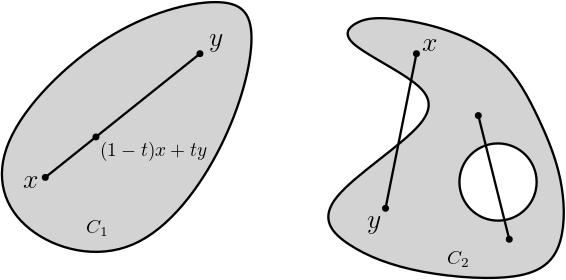
\includegraphics[width=0.60\textwidth]{conjuntos_convexo_naoconvexo}
	\caption{ Conjunto convexo e não-convexo. \label{fig:conjuntos_convexos}}
\end{figure}


Alguns exemplos de conjuntos convexos são o conjunto vazio, o espaço $\RR^{n}$, qualquer hiperplano do $\RR^{n}$ e um conjunto que contém um ponto só. A seguir, apresentamos alguns resultados importantes da análise convexa.

%{\cite[p. 50]{Ademir2013}}
\begin{lema} \label{lema:1_convexidade}
Considere $\Vert \cdot \Vert$ a norma euclidiana em $\RR^{n}$. Sejam $u,v \in \RR^{n}$ com $u\neq v$. Se $\Vert u \Vert = \Vert v \Vert = r$, então $\Vert (1-t)u + tv \Vert < r$, para todo $t \in (0,1)$.
\end{lema}

\begin{proof}
Seja $t \in (0,1)$ e suponha que $\Vert u \Vert = \Vert v \Vert = r$. Aplicando a desigualdade triangular, temos
\[
\Vert (1-t)u + tv \Vert \leq (1-t)\Vert u \Vert + t\Vert v \Vert = (1-t)r + tr = r.
\]
Agora, suponha por absurdo que $\Vert (1-t)u + tv \Vert = r$. Então
\[ \label{eq:1_lema1_convexidade}
(1-t)^{2} u^{T}u + 2t(1-t)u^{T}v + t^{2}v^{T}v = \Vert (1-t)u + tv \Vert^{2} = r^{2}.
\]
Como $u^{T}u = v^{T}v = r^{2}$ e $t \in (0,1)$, substituindo em \eqref{eq:1_lema1_convexidade} e desenvolvendo, obtemos 
\begin{align}
r^{2} &= (1-2t+t^{2}) u^{T}u + (2t-2t^{2})u^{T}v + t^{2}v^{T}v \\
&= (1-2t+t^{2}) r^{2} + (2t-2t^{2})u^{T}v + t^{2}r^{2} \\
&= r^{2} - 2tr^{2} + t^{2}r^{2} + (2t-2t^{2})u^{T}v + t^{2}r^{2} .
\end{align}
Evidenciando $r^{2}$, temos
\[ 
(2t-2t^{2})r^{2} = (2t-2t^{2})u^{T}v,
\]
e, portanto,
\[ \label{eq:2_lema1_convexidade}
r^{2} = u^{T}v.
\]
Assim, por \eqref{eq:2_lema1_convexidade},
\[
\Vert u-v \Vert^{2} = u^{T}u - 2u^{T}v + v^{T}v = r^{2} - 2r^{2} + r^{2} = 0,
\]
o que é uma contradição, pois por hipótese $u \neq v$. 
Portanto, concluímos que $\Vert (1-t)u + tv \Vert < r$, para todo $t \in (0,1)$.
\end{proof}

Agora, dado um conjunto $S \subset \RR^{n}$ e um ponto $z \in \RR^{n}$, considere o problema de encontrar um ponto de $S$ mais próximo de $z$, em outras palavras, queremos minimizar a distância de um ponto a um conjunto. Assim, os próximos resultados garantem a existência da solução no caso de $S$ ser um conjunto fechado e sua unicidade se, além de fechado, $S$ for convexo. Tal solução é chamada de projeção de $z$ sobre $S$, e denotada por $\proj_{S} (z)$. 

\begin{lema} \label{lema:existencia_projecao}
Seja $S \subset \RR^{n}$ um conjunto fechado não vazio. Dado $z \in \RR^{n}$, existe $\bar{z} \in S$ tal que
\[
\Vert z - \bar{z} \Vert \leq \Vert z - x \Vert,
\]
para todo $x \in S$.
\end{lema}
\begin{proof}
Seja $\alpha = \inf \{\Vert z-x \Vert \mid x \in S\}$. Então, para cada $n \in \mathds{N}$, existe $x^{n} \in S$ tal que
\[ \label{eq:1_lema_existencia_projecao}
\alpha \leq \Vert z-x^{n} \Vert \leq \alpha + \dfrac{1}{n}. 
\]
Em particular, $\Vert z-x^{n} \Vert \leq \alpha + 1$, para todo $n \in \mathds{N}$. Logo, existe uma subsequência $(x^{n^{k}})$ convergente, com $k \in \mathds{N}'$, tal que $x^{n^{k}} \longrightarrow \bar{z}$. Como $S$ é fechado temos que $\bar{z} \in S$. Além disso, 
\[
\Vert z-x^{n} \Vert \longrightarrow \Vert z-\bar{z} \Vert .
\]
Mas, por \eqref{eq:1_lema_existencia_projecao}, temos que $\Vert z-x^{n} \Vert \longrightarrow \alpha $, e portanto, concluímos que $\Vert z-\bar{z} \Vert = \alpha$.

\end{proof}


\begin{lema}  \label{lema:unicidadeprojecao_convexidade}
Seja $S \subset \RR^{n}$ um conjunto não vazio, convexo e fechado. Dado $z \in \RR^{n}$, existe um único $\bar{z} \in S$ tal que
\[
\Vert z - \bar{z} \Vert \leq \Vert z - x \Vert
\]
para todo $x \in S$.
\end{lema}
\begin{proof}
A existência é garantida pelo \Cref{lema:existencia_projecao}. Para provar a unicidade suponha que existam $\bar{z}, \tilde{z} \in S$, com $\bar{z} \neq \tilde{z}$, ta{}is que
\[ \label{eq:1_lema_unicidade_projecao}
\Vert z-\bar{z} \Vert \leq \Vert z-x \Vert \quad \text{e} \quad \Vert z-\tilde{z} \Vert \leq \Vert z-x \Vert ,
\]
para todo $x \in S$. Tomando $x=\tilde{z}$ na primeira desigualdade e $x=\bar{z}$ na segunda, obtemos
\[
\Vert z-\bar{z} \Vert = \Vert z-\tilde{z} \Vert .
\]
Por outro lado, o ponto $z^{*} = \dfrac{\bar{z} - \tilde{z}}{2}$ pertence ao conjunto convexo $S$. Além disso, pelo \Cref{lema:1_convexidade}, com $r= \Vert z-\bar{z} \Vert = \Vert z - \tilde{z} \Vert$ e $t=1/2$, temos
\begin{align}
\Vert z-z^{*} \Vert &=  \Vert z-t(\bar{z}+\tilde{z}) \Vert \\
& = \Vert z - t\bar{z} - t\tilde{z} \Vert \\
& = \Vert (1-t)(z-\bar{z}) + t(z-\tilde{z}) \Vert \\
& < r ,
\end{align}
o que é uma contradição, pois por \eqref{eq:1_lema_unicidade_projecao} teríamos
\[
r = \Vert z-\bar{z} \Vert = \Vert z - \tilde{z} \Vert \leq \Vert z-z^{*} \Vert < r .
\]
Portanto, $\bar{z} = \tilde{z}$.
\end{proof}


No \Cref{lema:unicidadeprojecao_convexidade} denotamos $\bar{z} = \proj_{S} (z)$.


\begin{teo}  \label{lema_condicaoprojecao_convexidade}
Sejam $S \subset \RR^{n}$ um conjunto não vazio, convexo e fechado, $z \in \RR^{n}$ e $\bar{z} = \proj_{S} (z)$. Então, 
\[
(z - \bar{z})^{T}(x - \bar{z}) \leq 0 ,
\]
para todo $x \in S$.
\end{teo}
\begin{proof}
Sejam $x \in S$ um ponto arbitrário e $\bar{z} = \proj_{S} (z)$. Pelo \Cref{lema:existencia_projecao} $\bar{z} \in S$ e, dado $t \in (0,1)$, pela convexidade de $S$, temos que $(1-t)\bar{z} + tx \in S$. Assim, 
\[
\Vert z-\bar{z} \Vert \leq \Vert z-(1-t)\bar{z} - tx \Vert = \Vert (z-\bar{z}) - t(x-\bar{z}) \Vert.
\]
Então, 
\[
\Vert z-\bar{z} \Vert^{2} \leq \Vert (z-\bar{z}) - t(x-\bar{z}) \Vert^{2} = \Vert z-\bar{z} \Vert^{2} - 2t(z-\bar{z})^{T}(x-\bar{z}) + t^{2}\Vert x- \bar{z} \Vert^{2} ,
\]
e como $t>0$, temos
\[ \label{eq:1_lema_condicaoprojecao_convexidade}
2(z-\bar{z})^{T}(x-\bar{z}) \leq t \Vert x- \bar{z} \Vert^{2} .
\]
Passando o limite em \eqref{eq:1_lema_condicaoprojecao_convexidade} quando $t\rightarrow 0$, obtemos
\[
(z-\bar{z})^{T}(x-\bar{z}) \leq 0, 
\]
completando a demonstração.
\end{proof}


O \Cref{lema_condicaoprojecao_convexidade} estabelece uma condição necessária e suficiente para caracterizar a projeção. Este resultado é provado no \Cref{lema:defineprojecao_convexidade}.


\begin{lema} \label{lema:defineprojecao_convexidade}
Sejam $S \subset \RR^{n}$ um conjunto não vazio, convexo e fechado e $z \in \RR^{n}$. Se $\bar{z} \in S$ satisfaz
\[
(z - \bar{z})^{T}(x - \bar{z}) \leq 0 ,
\]
para todo $x \in S$, então $\bar{z} = \proj_{S} (z)$.
\end{lema}
\begin{proof}
Dado $x\in S$ arbitrário, temos
\begin{align}
\Vert z-\bar{z} \Vert^{2} - \Vert z-x \Vert^{2} & = z^{T}z - 2z^{T}\bar{z} + \bar{z}^{T}\bar{z} - z^{T}z + 2z^{T}x - x^{T}x \\
& = - 2z^{T}\bar{z} + \bar{z}^{T}\bar{z} + 2z^{T}x - x^{T}x \\
& = (x-\bar{z})^{T}(2z-x-\bar{z}) \\
& = (x-\bar{z})^{T}(2(z-\bar{z})-(x-\bar{z})) \\
& = 2(x-\bar{z})^{T}(z-\bar{z}) - (x-\bar{z})^{T}(x-\bar{z}) \\
& \leq 0 .
\end{align}
pois $(x-\bar{z})^{T}(z-\bar{z}) \leq 0$ por hipótese, e $(x-\bar{z})^{T}(x-\bar{z}) = \Vert (x-\bar{z}) \Vert \geq 0$.
Logo,
\[
\Vert z-\bar{z} \Vert^{2} - \Vert z-x \Vert^{2} \leq 0,
\]
e, então
\[
\Vert z-\bar{z} \Vert^{2} \leq \Vert z-x \Vert^{2} ,
\]
para todo $x\in S$. Portanto, $\bar{z} = \proj_{S} (z)$.
\end{proof}


O \Cref{lema:defineprojecao_convexidade} fornece uma condição necessária de otimalidade ao minimizar uma função em um conjunto convexo fechado.


\begin{lema} \label{lema:associa_projecao_minimizador}
Sejam $f: \RR^{n} \rightarrow \RR$ uma função diferenciável e $C \subset \RR^{n}$ um conjunto convexo e fechado. Se $x^{*} \in C$ é minimizador local de $f$ em $C$, então
\[
\proj_{C} (x^{*} - \alpha \nabla f(x^{*})) = x^{*} ,
\]
para todo $\alpha \geq 0$.
\end{lema}
\begin{proof}
Seja $x^{*} \in C$ minimizador local de $f$ em $C$. Fixando $x\in C$, como $C$ é um conjunto convexo, temos
\[ \label{eq:1_lema_associa_projecao_minimizador}
f(x^{*}) \leq f((1-t)x^{*} + tx),
\]
para todo $t\geq 0$ suficientemente pequeno. Pelo \Cref{fato:Taylor_primeira_ordem}, 
\[ \label{eq:2_lema_associa_projecao_minimizador}
f(x^{*}+t(x-x^{*})) = f(x^{*}) + t\nabla f(x^{*})^{T}(x-x^{*}) + o(t) ,
\]
em que $\lim_{t\rightarrow 0} \dfrac{o(t)}{t} = 0$. Dessa forma, por \eqref{eq:1_lema_associa_projecao_minimizador} e \eqref{eq:2_lema_associa_projecao_minimizador}, temos
\[
0 \leq f(x^{*}+t(x-x^{*})) - f(x^{*}) = t\nabla f(x^{*})^{T}(x-x^{*}) + o(t) ,
\]
e portanto, 
\[ \label{eq:3_lema_associa_projecao_minimizador}
t\nabla f(x^{*})^{T}(x-x^{*}) + o(t) \geq 0.
\]
Dividindo por $t$ e passando o limite quando $t \rightarrow 0$ em \eqref{eq:3_lema_associa_projecao_minimizador}, obtemos
\[
\nabla f(x^{*})^{T}(x-x^{*}) \geq 0.
\]
Assim, dado $\alpha \geq 0$,
\[
(x^{*} - \alpha \nabla f(x^{*}) - x^{*})^{T}(x-x^{*}) = -\alpha \nabla f(x^{*})^{T}(x-x^{*}) \leq 0,
\]
para todo $x\in C$. Portanto, pelo \Cref{lema:defineprojecao_convexidade} concluímos que $\proj_{C} (x^{*} - \alpha \nabla f(x^{*})) = x^{*}$, para todo $\alpha \geq 0$.
\end{proof}


%----------------------------------------------------------------------------------------------------------------------------


\subsection{Funções Convexas}

\begin{defi} \label{defi:funcao_convexa}
Seja $C \subset \RR^{n}$ um conjunto convexo. Dizemos que a \emph{função} $f: \RR^{n} \rightarrow \RR$ é \emph{convexa} em $C$ quando
\[
f((1-t)x + ty) \leq (1-t)f(x) + tf(y),
\]
para todos $x,y \in C$ e $t \in [0,1]$.

Se para todo $t \in (0,1)$ e $x \neq y$ vale que
\[
f((1-t)x + ty) < (1-t)f(x) + tf(y),
\]
dizemos que $f$ é \emph{estritamente convexa}.
\end{defi}
A \Cref{fig:funcao_convexa} apresenta um exemplo de uma função convexa, enquanto que na \Cref{fig:funcao_nao_convexa} podemos vizualizar uma função não-convexa.

\begin{figure}[!ht] 
\centering
\begin{subfigure}[h]{0.42\textwidth}
\centering
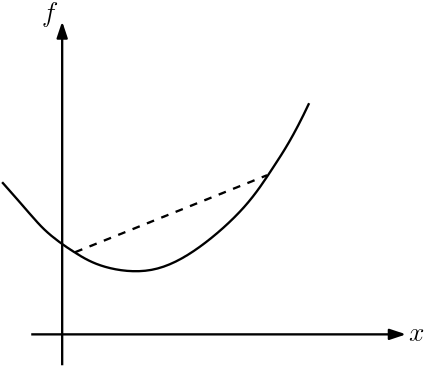
\includegraphics[width=\textwidth]{funcao_convexa_1}
\caption{Função Convexa \label{fig:funcao_convexa}}
\end{subfigure}
\begin{subfigure}[!ht]{0.40\textwidth}
	\centering
	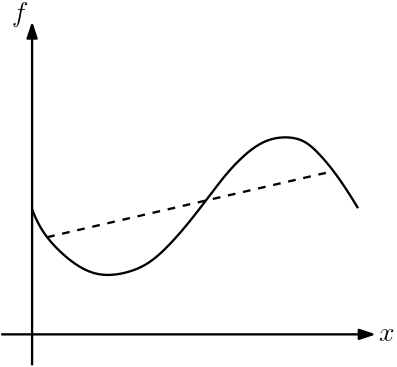
\includegraphics[width=\textwidth]{funcao_nao_convexa}
	\caption{Função não convexa. \label{fig:funcao_nao_convexa}}
\end{subfigure}
\caption{Funções convexas e não-convexas. \label{fig:exemplos_funcao_convexa}}
\end{figure}

A noção geométrica da \Cref{defi:funcao_convexa} é apresentada na \Cref{fig:nocao_funcao_convexa}, em que qualquer arco do gráfico de uma função convexa está sempre abaixo do segmento que liga as extremidades.

\begin{figure}[!ht] 
	\centering
	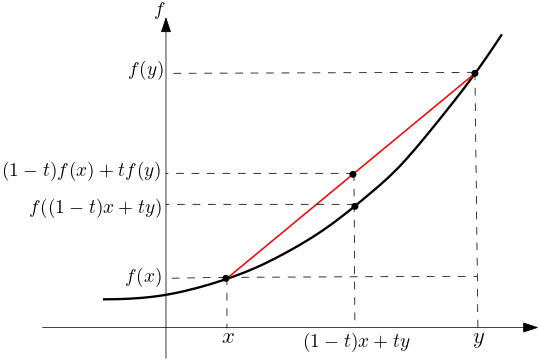
\includegraphics[width=0.75\textwidth]{nocao_geometrica_funcao_convexa}
	\caption{Noção geométrica de uma função convexa. \label{fig:nocao_funcao_convexa}}
\end{figure}

\begin{defi}
Se $C \subset \RR^{n}$ é um conjunto convexo, dizemos que $f: C \rightarrow \RR $ é uma \emph{função côncava} em $C$, quando a função $(-f)$ é convexa em $C$.
\end{defi}

Assim, maximizar uma função côncava num conjunto convexo equivale a minimizar uma função convexa num conjunto convexo.

O \Cref{teo:convexidade_e_minimizador} justifica o fato da convexidade ser uma propriedade tão importante em otimização.

\begin{teo} \label{teo:convexidade_e_minimizador}
Sejam $C \subset \RR^{n}$ um conjunto convexo e $f:C \rightarrow \RR$ uma função convexa. Se $x^{*} \in C$ é minimizador local de $f$, então $x^{*}$ é minimizador global de $f$.
\end{teo}
\begin{proof}
Seja $x^{*}$ um minimizador local de $f$. Então, existe $\delta > 0$ tal que 
\[
f(x^{*}) \leq f(x), 
\]
para todo $x \in B(x^{*}, \delta) \cap C$. Considere $y \in C$, tal que $y \notin B(x^{*}, \delta)$, e tome $t \in (0,1]$ de modo que $t \Vert y-x^{*} \Vert < \delta$. Assim, o ponto $x = (1-t)x^{*} + ty$ satisfaz
\[
\Vert x - x^{*} \Vert = \Vert (1-t)x^{*} + ty - x^{*} \Vert = \Vert x^{*} - tx^{*} + ty - x^{*} \Vert = t \Vert y - x^{*} \Vert < \delta ,
\]
e, portanto, $x \in B(x^{*}, \delta) \cap C$.
Desse modo, como $f$ é uma função convexa, temos
\[
f(x^{*}) \leq f(x) \leq (1-t)f(x^{*}) + tf(y) = f(x^{*}) + t(f(y)-f(x^{*})),
\]
donde segue que $f(x^{*}) \leq f(y)$.
Portanto, $x^{*}$ é minimizador global de $f$.
\end{proof}

A seguir apresentamos outra forma de caracterizar a convexidade de uma função quando temos hipóteses de diferenciabilidade.

\begin{teo}  \label{teo:diferenciabilidade_e_convexidade}
Sejam $f: \RR^{n} \rightarrow \RR $ uma função diferenciável e $C \in \RR^{n}$ um conjunto convexo. A função $f$ é convexa em $C$ se, e somente se, 
\[
f(y) \geq f(x) + \nabla f(x)^{T}(y-x),
\]
para todos $x, y \in C$.
\end{teo}


\begin{proof}
Seja $f$ uma função convexa. Para $x,y \in C$ e $t \in (0,1]$ quaisquer, temos $(1-t)x + ty = x + t(y-x)$. Assim, definindo $d = y-x$, temos que $x + td \in C$ e
\[
f(x+td) = f((1-t)x + ty) \leq (1-t)f(x) + tf(y),
\]
logo
\[
f(x+td) \leq f(x) + t(f(y)-f(x)),
\]
o que implica em 
\[
f(y)-f(x) \geq \dfrac{f(x+td)-f(x)}{t} .
\]
Passando o limite quando $t \rightarrow 0^{+}$, temos
\[
f(y)-f(x) \geq \lim_{t \rightarrow 0^{+}} \dfrac{f(x+td)-f(x)}{t} = \nabla f(x)^{T} d = \nabla f(x)^{T} (y-x) ,
\]
e, portanto,
\[
f(y) \geq f(x) + \nabla f(x)^{T} (y-x) .
\]

Reciprocamente, considere $z = (1-t)x + ty$ e observe que 
\[
f(x) \geq f(z) + \nabla f(z)^{T}(x-z) \quad \text{e} \quad f(y) \geq f(z) + \nabla f(z)^{T}(y-z) .
\]
Agora, multiplicando a primeira desigualdade por $(1-t)$ e a segunda por $t$, obtemos
\begin{align}
(1-t)f(x) + tf(y) & \geq (1-t)(f(z) + \nabla f(z)^{T}(x-z)) + t(f(z) + \nabla f(z)^{T}(y-z)) \\
& \geq f(z) + \nabla f(z)^{T}(x-z) - tf(z) -t\nabla f(z)^{T}(x-z) + tf(z) + t\nabla f(z)^{T}(y-z) \\
& \geq f(z) + \nabla f(z)^{T}(x-z) + t\nabla f(z)^{T}(-x+z+y-z) \\
& \geq f(z) + \nabla f(z)^{T}(x-z) + t\nabla f(z)^{T}(y-x) \\
& \geq f(z) + \nabla f(z)^{T}(x-z) + t\nabla f(z)^{T} \dfrac{(z-x)}{t} \\
& \geq f(z) + \nabla f(z)^{T}(x-z) - \nabla f(z)^{T}(x-z) \\
& = f(z) \\
& = f((1-t)x + ty) .
\end{align}
Portanto, a função $f$ é convexa em $C$.
\end{proof}

O \Cref{teo:diferenciabilidade_e_convexidade} afirma que a aproximação linear baseada na derivada local subestima a função convexa. Este resultado é ilustrado na \Cref{fig:funcao_convexa_aproximacao_linear_derivada} a seguir. 
\begin{figure}[!ht] 
	\centering
	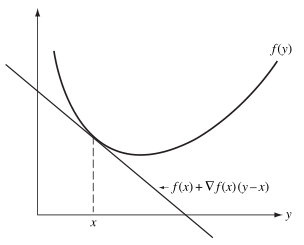
\includegraphics[width=0.50\textwidth]{funcao_convexa_aproximacao_linear_derivada}
	\caption{Ilustração da \Cref{teo:diferenciabilidade_e_convexidade}. \label{fig:funcao_convexa_aproximacao_linear_derivada} \\ Fonte: \textcite{luenberger2008linear}}
\end{figure}

Para os resultados que vem a seguir vamos utilizar o \Cref{fato:Taylor_com_resto_lagrange}, que fornece a fórmula de Taylor com resto de Lagrange. Sua demonstração pode ser encontrada em \textcite[p.196]{Elon2019}.

\begin{fato}(\textbf{Taylor com Resto de Lagrange}) \label{fato:Taylor_com_resto_lagrange}
Considere $f: \RR^{n} \rightarrow \RR$ uma função de classe $\mathcal{C}^{1}$ e $\xbar, d \in \RR^{n}$. Se $f$ é duas vezes diferenciável no segmento $(\xbar , \xbar + d)$, então existe $t \in (0,1)$ tal que
\[
f(\xbar + d) = f(\xbar) + \nabla f(\xbar)^{T} d + \dfrac{1}{2}d^{T}\nabla^{2} f(\xbar + td)d .
\]
\end{fato}


\begin{lema} \label{lema:auxiliar_para_teo_hessiana_convexidade}
Sejam $C \subset \RR^{n}$ convexo, $x \in \bar{C}$ e $y \in \interior C$. Então, $(x,y] \subset \interior C$.
\end{lema}
\begin{proof}
Por demonstrar.
\end{proof}


\begin{teo} \label{teo:hessiana_convexidade}
Sejam $f:\RR^{n} \rightarrow \RR $ uma função de classe $\mathcal{C}^{2}$ e $C \subset \RR^{n}$ um conjunto convexo com interior não vazio. A função $f$ é convexa em $C$ se, e somente se, a Hessiana $\nabla^{2} f(x)$ é semidefinida positiva para todo $x \in C$.
\end{teo}
\begin{proof}
Considere $x \in \interior C$. Então, dado $d \in \RR^{n}$ temos que $x+td \in C$, para $t$ suficientemente pequeno. Portanto, pela convexidade de $f$ e pelo \Cref{teo:diferenciabilidade_e_convexidade}, temos
\[
f(x+td) \geq f(x) + t\nabla f(x)^{T} d ,
\]
e assim, 
\[ \label{eq:1_teo_hessiana_convexidade}
f(x+td) -f(x) - t\nabla f(x)^{T} d \geq 0 . 
\]
Aplicando o \Cref{fato:Taylor_segunda_ordem} para $f(x+td)$, temos
\[
f(x+td) = f(x) + t\nabla f(x)^{T}d + \dfrac{t^{2}}{2}d^{T} \nabla^{2} f(x)d + o(t^{2}) ,
\]
e substituindo em \eqref{eq:1_teo_hessiana_convexidade}, obtemos
\[
\dfrac{t^{2}}{2}d^{T} \nabla^{2} f(x)d + o(t^{2}) \geq 0 ,
\]
com $\lim_{t \rightarrow 0} \dfrac{o(t^{2})}{t^{2}} = 0$. 
Dividindo por $t^{2}$ e passando o limite com $t \rightarrow 0$, temos
\[
d^{T} \nabla^{2} f(x)d \geq 0 .
\]
Agora, considere $x \in C$ arbitrário. Como existe $y \in \interior C$, o \Cref{lema:auxiliar_para_teo_hessiana_convexidade} garante que todos os pontos do segmento $(x,y] \subset \interior C$. Então, pelo que acabamos de provar, dados $d \in \RR^{n}$ e $t\in (0,1]$, vale
\[
d^{T} \nabla^{2} f((1-t)x+ty)d \geq 0 .
\]
Fazendo $t \rightarrow 0^{+}$ e usando a continuidade de $\nabla^{2} f$, obtemos
\[
d^{T} \nabla^{2} f(x)d \geq 0,
\]
para todo $x \in C$.

Reciprocamente, dados $x \in C$ e $d \in \RR^{n}$ tal que $x+d \in C$, pelo \Cref{fato:Taylor_com_resto_lagrange},
\[
f(x+d) = f(x) + \nabla f(x)^{T}d + \dfrac{1}{2}d^{T} \nabla^{2} f(x+td)d,
\]
para algum $t \in (0,1)$. Como $\nabla ^{2}f(x+td) \geq 0$, concluímos que 
\[
f(x+d) \geq f(x) + \nabla f(x)^{T}d .
\]
Logo, pelo \Cref{teo:diferenciabilidade_e_convexidade}, $f$ é convexa.
\end{proof}

Tendo em vista que a função objetivo dos problemas de SVM são funções quadráticas, é necessário avaliar sob quais condições uma função quadrática é convexa. Tal resultado é apresentado a seguir e sua demonstração decorre do \Cref{teo:hessiana_convexidade}.

%\cite{Gondzio2018}
\begin{teo} \label{teo:funcao_quadratica_e_convexa}
Seja $C \in \RR^{n}$ um conjunto convexo e $Q \in \RR^{n\times n}$ uma matriz quadrada e simétrica. Seja $f:C \rightarrow \RR$ tal que $f(x) = x^{T}Qx$ é uma função quadrática. Então, $f$ é convexa se, e somente se, $Q$ é semidefinida positiva.
\end{teo}
\begin{proof}
Primeiramente, suponhamos que $f$ é convexa em $C$. Então, pelo \Cref{teo:hessiana_convexidade}, a Hessiana $\nabla^{2} f(x)$ é semidefinida positiva para todo $x\in C$, e como $\nabla^{2} f(x) = 2Q$, concluímos que $Q$ é semidefinida positiva. Reciprocamente, se $\nabla^{2} f(x) = 2Q$ é semidefinida positiva, então, pelo \Cref{teo:hessiana_convexidade}, a função $f$ é convexa em $C$.
\end{proof}

Desse modo, nos problemas de minimização irrestrita em que a função objetivo é uma quadrática da forma
\[
f(x) = \dfrac{1}{2}x^{T}Qx - b^{T}x,
\]
com $Q\in \RR^{n\times n}$ simétrica e $b\in \RR^{n}$, 
temos que se $x^{*}$ é mínimo local de $f$ então, pelas condições necessárias de otimalidade, \Cref{teo:condicao_necessaria_1_ordem,teo:condicao_necessaria_2_ordem}, devemos ter
\[
\nabla f(x^{*})= Qx^{*}-b =0 \quad \text{e} \quad \nabla^{2} f(x^{*})=Q \succcurlyeq 0.
\]
Logo, se $Q$ é semidefinida positiva, pelo \Cref{teo:funcao_quadratica_e_convexa} $f$ é convexa, e pelo \Cref{teo:convexidade_e_minimizador} qualquer ponto $x^{*}$ que satisfaça a condição de otimalidade de primeira ordem 
\[ \label{eq:condicao_1_ordem_quadratica_convexidade}
\nabla f(x^{*})= Qx^{*}-b =0
\] 
é um minimizador global de $f$. Por outro lado, cabe ressaltar que pode não existir solução para a equação \eqref{eq:condicao_1_ordem_quadratica_convexidade} se $Q$ é singular. No entanto, temos que se $Q$ é definida positiva então $Q$ é invertível, e resolvendo a equação \eqref{eq:condicao_1_ordem_quadratica_convexidade} o vetor
\[
x^{*} = Q^{-1}b
\]  
é o único mínimo global.

Além de quadrática, a função objetivo do problema de classificação \eqref{eq:problemageralSVM} envolve a norma de um vetor $w \in \RR^{n}$. Em vista disso, a proposição a seguir garante a convexidade da norma.

\begin{prop} \label{prop:norma_funcao_convexa}
Considere a função $f: \RR^{n} \rightarrow \RR$ dada por
\[
f(x) = \dfrac{1}{2}\Vert x \Vert,
\]
com $x\in \RR^{n}$. Então a função $f$ é uma função convexa.
\end{prop}
\begin{proof}
Seja $\Vert \cdot \Vert$ a norma de um vetor. Para quaisquer $x, y \in \RR^{n}$ e qualquer $\alpha \in [0,1]$, temos que
\begin{align}
f(\alpha x + (1-\alpha)y) &= \dfrac{1}{2} \Vert \alpha x + (1-\alpha)y \Vert \\
&\leq \dfrac{1}{2} \Vert \alpha x\Vert + \dfrac{1}{2}\Vert (1-\alpha)y \Vert \\
&= \alpha \dfrac{1}{2} \Vert x \Vert + (1-\alpha)\dfrac{1}{2} \Vert y \Vert \\
&= \alpha f(x) + (1-\alpha)f(y).
\end{align}
Portanto, $f$ é uma função convexa.
\end{proof}

\newpage

\printbibliography
\end{document}